\documentclass{article}
\usepackage{import}

\usepackage{amsmath}
\usepackage{amssymb}
\usepackage{amsfonts}
\usepackage{mathtools}

\usepackage[thmmarks, amsmath]{ntheorem}

\usepackage{graphicx}
\usepackage{xcolor}
\usepackage{float}

\usepackage{tikz}
\usetikzlibrary{arrows, positioning}
\usepackage{tikz-cd}

\usepackage{diffcoeff}
\diffdef{}{op-symbol=\mathrm{d},op-order-sep=0mu,}
\diffdef{p}{left-delim=\left.,right-delim=\right|,subscr-nudge=0mu}

\usepackage{cancel}
\usepackage{interval}
\usepackage{mleftright}

\usepackage[inline]{enumitem}
\SetEnumitemKey{algorithm}{label={Step \Roman*.}, labelindent=0pt, labelsep=!, leftmargin=*, align=left,itemindent=0pt}
\setlist[enumerate,1]{label=\roman*)}

\usepackage{cite}

\usepackage{showlabels}


\title{A Short Introduction to Hamiltonian Persistence Homology}
\author{Duarte Maia}
%\date{}

\theorembodyfont{\upshape}
\theoremseparator{.}
\newtheorem{theorem}{Theorem}
\newtheorem{prop}{Proposition}
\newtheorem{corollary}{Corollary}
\renewtheorem*{prop*}{Prop}
\newtheorem{lemma}{Lemma}
\newtheorem{definition}{Definition}
\newtheorem{remark}{Remark}

\theoremstyle{nonumberplain}
\theoremheaderfont{\itshape}
\theorembodyfont{\upshape}
\theoremseparator{:}
\theoremsymbol{\ensuremath{\blacksquare}}
\newtheorem{proof}{Proof}

\theoremsymbol{\ensuremath{\text{\textit{(End proof of lemma)}}}}
%\theoremsymbol{\ensuremath{\square}}
\newtheorem{lemmaproof}{Proof of lemma}

%Sets of numbers
\newcommand{\R}{\mathbb{R}}
\newcommand{\C}{\mathbb{C}}
\newcommand{\Z}{\mathbb{Z}}

\newcommand{\FF}{\mathbb{F}} %Arbitrary field

%Contractible orbits
\newcommand{\LL}{\mathrm{L}}
%Action functional
\renewcommand{\AA}{\mathrm{A}}
%Generic Barcode
\newcommand{\BB}{\mathrm{B}}

%Floer Complex and Homology
\newcommand{\CF}{\mathrm{CF}}
\newcommand{\HF}{\mathrm{HF}}

\newcommand{\moduli}{M}

%Morse Complex
\newcommand{\MC}{\mathrm{C}}

\DeclareMathOperator{\Ind}{Ind}
\DeclareMathOperator{\hessian}{Hess}

\newcommand{\I}{\mathrm{i}}
\newcommand{\e}{\mathrm{e}}


\DeclareMathOperator{\sign}{sign}
\let\Im\relax
\DeclareMathOperator{\Im}{Im}
\let\Re\relax
\DeclareMathOperator{\Re}{Re}

\newcommand{\Ix}{\mathop{\mathrm{I\mkern0.7mu x}}}
%\newcommand{\Ix}{\mathop{\mathrm{ix}}}


\newcommand{\id}{\mathrm{id}}

\DeclareMathOperator{\image}{im}


\DeclareMathOperator{\inte}{int}
\DeclareMathOperator{\codim}{codim}
\newcommand{\grad}{\nabla}
\newcommand{\into}{\mathbin{\lrcorner}}

\DeclarePairedDelimiter{\norm}{\lvert}{\rvert}
\DeclarePairedDelimiter{\Norm}{\lVert}{\rVert}
\DeclarePairedDelimiter{\abs}{\lvert}{\rvert}
\DeclarePairedDelimiter{\braket}{\langle}{\rangle}

\newcommand{\conj}[1]{\overline{#1}}
\newcommand{\transposed}{\top}
\DeclareMathOperator{\trace}{Tr}

%conley zehnder index a la hofer and kriener
\newcommand{\muhk}{\mu_{\mathrm{HK}}}

\includeonly{
%introduction,
%ph101,
%barcodesfromffh,
%firstexample1,
maslov,
%firstexample2,
%secondexample
}

\begin{document}
\maketitle

\pagebreak

\tableofcontents

\pagebreak

% !TeX root = Thesis.tex

\chapter{Introduction}

\paragraph{Persistence Homology}
Persistence Homology is a relatively recent area of mathematics. It was borne from the need to approximate homology of spaces in data science, but flourished into a tool applicable to many areas of mathematics, including differential and symplectic geometry. For a historical overview see \cite{historypersistence}. For a recent exposition of persistence homology applied to geometry and topological function theory see \cite{polterovich}.

To understand persistence homology, it is instructive to look at a concrete example. Consider a torus embedded vertically in $\R^3$ as in figure \ref{fig:torus1}, with the critical values of the height function at 
$z_1 < z_2 < z_3 < z_4$. Classical homology (which does not care how the torus is embedded in $\R^3$) tells us that the torus has one connected component, two holes in dimension 1, and one hole in dimension 2. Persistence homology goes further, by telling us roughly where these holes are located.

\begin{figure}
\centering
\begin{tikzpicture}
\draw[->] (-2,-3) -- (-2,3.5) node[right] {$z$};

\draw (0,0) ellipse (1.5 and 2.7);
  \begin{scope}
    \clip (1.4,0) ellipse (1.8 and 3);
    \draw[name path global=p1] (-1,0) ellipse (1.2 and 2);
  \end{scope}
  \begin{scope}
    \clip (-1,0) ellipse (1.2 and 2);
    \draw[name path global=p2] (1,0) ellipse (1.2 and 2);
  \end{scope}
  
  
\draw[dashed] (0, 2.7) -- (-1.9, 2.7);
\draw (-1.9,2.7) -- (-2.1,2.7) node[left] {$z_4$};

\draw[dashed] (0, -2.7) -- (-1.9, -2.7);
\draw (-1.9,-2.7) -- (-2.1,-2.7) node[left] {$z_1$};

\node (origin) at (0,0) {};
\node (tr) at (-1.9,0) {};
\node (tl) at (-2.1,0) {};


\path [name intersections={of=p1 and p2}];


\draw[dashed] (origin |- intersection-1) -- (tr |- intersection-1);
\draw (tr |- intersection-1) -- (tl |- intersection-1) node[left] {$z_3$};

\draw[dashed] (origin |- intersection-2) -- (tr |- intersection-2);
\draw (tr |- intersection-2) -- (tl |- intersection-2) node[left] {$z_2$};


\end{tikzpicture}
\caption{An embedding of a torus in $\R^3$}\label{fig:torus1}
\end{figure}

Define $X_t$, for $t \in \R$, as the subset of the torus $T$ given by
\begin{equation}
X_t = \{ (x,y,z) \in T \mid z < t \}.
\end{equation}

This is an example of a \emph{filtration of the torus}: a decomposition of $T$ as an increasing union of suitable spaces. If we compute, say, the first homology of the spaces $X_t$, we get a family of modules
\begin{equation}
V_t = H_1(X_t), t \in \R,
\end{equation}
which give us far more information that $H_1(T)$ alone.

From this point onward, we restrict our attention to the case of homology with coefficients in a field $\FF$, as the theory on persistence homology over other rings is much sparser.

The inclusion maps $i_{ts} \colon X_t \hookrightarrow X_s$ for $t \leq s$ induce linear maps $\pi_{ts} \colon V_t \to V_s$, and these maps satisfy the equation
\begin{equation}
\pi_{sr} \circ \pi_{ts} = \pi_{tr}, \quad t < s < r,
\end{equation}
as well as $\pi_{tt} = \id$. Such a collection of data (a real-indexed family of vector spaces and maps $\pi_{ts}$ as above) is called a \emph{persistence module} and besides giving us information on the topological features of the space, it gives us an idea of where they are located.

Let us look at the example of the torus from figure \ref{fig:torus1}. Its persistence homology is (up to isomorphism) given by the following description. For $t \leq z_1$, $X_t$ is empty, and for $z_1 < t \leq z_2$, $X_t$ is homeomorphic to a disk. Therefore, for $t \leq z_2$, $X_t = \{0\}$. At $t = z_2$, the disk suddenly becomes closed, so $V_t$ becomes isomorphic to $\FF$. Finally, at $t = z_3$ the second handle is closed, so $V_t$ becomes $\FF^2$.

This concludes the computation of the spaces $V_t$, but it is also necessary to specify the linear maps $\pi_{ts} \colon V_t \to V_s$. In this case, it is easy to check that they are the inclusions $\FF^n \hookrightarrow \FF^m$, where $m$ and $n$ are as appropriate. Thus, we have the persistence module of first homology the torus $T$ (associated to the particular embedding from figure \ref{fig:torus1}), but we do not yet have a good representation for it.

Enter barcodes and the Normal Form Theorem. A barcode is a simple combinatorial object, given by a finite multiset\footnote{This is a set whose elements are counted with multiplicity} of intervals in $\R$. To each barcode $B$ is associated a persistence module denoted $\FF(B)$. It is a surprising fact that, under reasonable finiteness assumptions (a module which satisfies them is said to be of \emph{finite type}), to each persistence module is associated a unique barcode:
\begin{theorem*}[Normal form theorem]
Let $V = (\{V_t\}_{t \in \R}, \{\pi_{ts}\}_{t\leq s})$ be a persistence module of finite type. Then, there exists a unique barcode $B$ such that $V$ is isomorphic to $\FF(B)$.
\end{theorem*}

This theorem may be applied to the persistence module of the torus computed before, yielding a barcode with two bars, which is represented in figure \ref{fig:bctorus}.

\begin{figure}
\centering
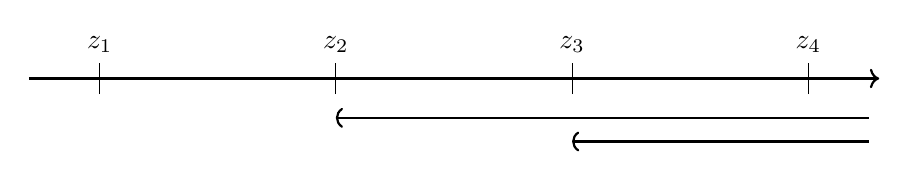
\begin{tikzpicture}[xscale=3]
\draw[->,thick] (-0.300,0.000)--(3.300,0.000);
\draw[] (0.000,-0.200)--(0.000,0.200) node[above] {$z_1$};
\draw[] (1.000,-0.200)--(1.000,0.200) node[above] {$z_2$};
\draw[] (2.000,-0.200)--(2.000,0.200) node[above] {$z_3$};
\draw[] (3.000,-0.200)--(3.000,0.200) node[above] {$z_4$};
\draw[(-,thick] (1.000,-0.500)--(3.255,-0.500) node[right] {};
\draw[(-,thick] (2.000,-0.800)--(3.255,-0.800) node[right] {};
\end{tikzpicture}
\caption{Visual representation of the barcode associated to the first homology of the torus in \ref{fig:torus1}.}\label{fig:bctorus}
\end{figure}

This correspondence is akin to a very familiar fact from linear algebra: every finite-dimensional vector space is uniquely identified by a single natural number, its dimension. Persistence modules are a bit more complicated than vector spaces, so they are represented by a more complex object, but it is still surprising that all the information in a (finite type) persistence module can be summarized in such a simple object.

\paragraph{Symplectic Geometry and Floer Homology}

Symplectic Geometry is technically not a recent area, with the first recorded instance of something akin to a symplectic structure being found in a 1809 paper by Lagrange; see \cite{marle2009inception} for an account of this and other contemporary papers using modern-day notation. However, the field had a large explosion following a 1985 article by Mikhail Gromov, after which symplectic geometry started absorbing methods from algebraic geometry, differential topology, and PDEs, especially with the introduction of a new type of homology by Andreas Floer.

The basic object of study of symplectic geometry is a symplectic manifold, which consists of a smooth manifold $M$ equipped with a rank-2 differential form $\omega$ which is non-degenerate.\footnote{For every vector $v$ tangent to $M$, there exists some $w$ tangent to the same point such that $\omega(v,w) \neq 0$.} This innocuous definition hides a large amount of complexity. For a brief introduction to the subject, see chapter 7 of \cite{polterovich}. For a slightly less brief introduction see chapter 5 of \cite{audin}, and for a standard textbook see \cite{mcduff}. For the remainder of the introduction, we will assume that the reader is familiar with basic concepts from symplectic geometry, such as almost-complex structures and Hamiltonian systems.

An important (now solved) problem in symplectic geometry, the Arnol'd conjecture, regards the number of periodic orbits of a Hamiltonian system on a symplectic manifold. The major breakthrough in proving the so-called Arnol'd conjecture was the introduction of Floer homology in 1988, but since then Floer homology has grown a life of its own.

Floer homology is a bit like a symplectic version of Morse theory: one begins with a (possibly time-dependent) Hamiltonian $H$ on a compact symplectic manifold\footnote{We also require a technical condition called \emph{asphericity}: the manifold $M$ must satisfy $\pi_2(M) = 0$, i.e. any continuous map $S^2 \to M$ must be homotopic to a constant map.} $(M,\omega)$ and counts the number of orbits of $H$ which are time-one periodic and contractible. These coincide with the critical points of a certain functional, called the \emph{action functional}, which is the start of the analogy between Floer and Morse homology: this functional $\AA$ takes the place that a Morse function would in Morse theory. Then to each such orbit one associates an integer, called the Maslov index, which takes the role of the Morse index and to which we dedicate the entirety of chapter \ref{chap:maslov}. Finally, with the help of an almost-complex structure $J$ on $M$ (which takes the role that a Riemannian metric would in Morse theory) one may define a boundary map $\partial \colon \CF_k(M,H) \to \CF_{k-1}(M,H)$, where $\CF_k(M,H)$ denotes the vector space (in a chosen field $\FF$) freely spanned by the time-one contractible periodic orbits of $H$ whose index is $k$. Like in Morse theory, this map is computed by counting the number of solutions to a certain differential equation which connect an orbit $\gamma$ of index $k$ and another orbit $\eta$ of index $k-1$. The main difference, which makes the theory much more intricate and heavy on analysis, is that while in Morse theory these connecting paths are solutions of a certain ODE, in Floer theory the paths connecting $\gamma$ and $\eta$ must satisfy a \emph{PDE}; these curves are said to be \emph{pseudo-holomorphic}. Interestingly, this PDE can also be interpreted as an ODE in the space of contractible loops, given by the flow of the negative gradient of the action functional $\AA$.

It is a surprising but well-known theorem that the Floer homology $\HF_k(M,H,J)$ (which is the homology associated to the complex $(\CF_k(M,H), \partial(M,H,J))$) does not depend on the chosen Hamiltonian $H$ or almost-complex structure $J$, and in fact agrees with the homology of $M$ in the usual sense (modulo a shift in index, depending on the conventions chosen for the Maslov index).

For an excellent introduction to the subject, including both Floer and Morse homology, see the outstanding book by Michèle Audin and Mihai Damian \cite{audin}.

\paragraph{Filtered Floer Homology}

We are now ready to unite Floer homology and persistence. The idea is to introduce a filtration, akin to the $X_t$ from the torus example above, but instead of filtering the space $M$, we filter the space of orbits.

Recall that Floer homology is the homology associated to a certain chain complex,
\begin{equation}
(\CF_k(M,H), \partial(M,H,J)),
\end{equation}
where the vector spaces $\CF_k(M,H)$ are spanned by periodic orbits of $H$. The action functional is defined on these orbits, and it is an elementary fact that
\begin{equation}\label{eq:actiondecrease}
\text{If $a \in \CF_k$, $b_1, \dots b_N \in \CF_{k-1}$, and } \partial(a) = \sum n_i b_i \text{ then } \forall_i \, \AA(b_i) < \AA(a).
\end{equation}

Therefore, if we filter the space of orbits by their action, the differential restricts nicely to the filtered spaces. In other words, if we define
\begin{equation}
\begin{gathered}
\CF_k^\lambda(M,H) = \braket{a \in \CF_k(M,H) \mid \AA(a) < \lambda},\\
\partial^\lambda = \partial|_{\CF_k^\lambda} \colon \CF_k^\lambda(M,H) \to \CF_{k-1}^\lambda(M,H),
\end{gathered}
\end{equation}
the differentials $\partial^\lambda$ are well-defined because of \eqref{eq:actiondecrease}.

This construction yields a real-indexed family of chain complexes, with an obvious chain map given by the inclusion $i_{st} \colon \CF_k^s \to \CF_k^t$ for $s \leq t$. This chain map passes to homology, which yields the so-called \emph{filtered Floer homology}, which is denoted by $\HF_k^\lambda(M,H,J)$, with $k \in \Z$ and $\lambda \in \R$, and is equipped with maps $\pi_{st} \colon \HF_k^s \to \HF_k^t$ for $s \leq t$. Unlike usual Floer homology, filtered Floer homology depends in general on the chosen Hamiltonian $H$, in the same way that the filtered homology of the torus shown in the beginning of the introduction depends on the chosen embedding of the torus in $\R^3$. However, it depends only on the time-one flow of $H$, so we can actually define the \emph{filtered Floer homology of a Hamiltonian diffeomorphism} $\phi$, denoted $\HF_k^\lambda(M,\phi)$, with associated maps $\pi_{ts} \colon \HF_k^t \to \HF_k^s$, $t<s$.

Applying the normal form theorem to the filtered Floer homology of a Hamiltonian diffeomorphism, we obtain a barcode (in each degree $k$) associated to a Hamiltonian diffeomorphism $\phi$, denoted $\BB_k(\phi)$. We may also construct the so-called \emph{total barcode of $\phi$},
\begin{equation}
\BB(\phi) = \bigcup_k \BB_k(\phi),
\end{equation}
and from here we may ask the question: `What properties of $\phi$ can we tell from its barcode?' 

This is an active area of research. Polterovich et al. \cite{polterovich} show that one can find estimates for Hofer's metric using the so-called \emph{bottleneck metric} on the space of barcodes, a subject upon which we will not touch here, and with it prove that Hofer's metric is nondegenerate for aspherical closed manifolds. Albers and Frauenfelder \cite{albers2014square} find a barcode-based necessary condition for a Hamiltonian diffeomorphism to be of the form $\psi \circ \psi$, with $\psi$ another Hamiltonian diffeomorphism. Usher \cite{usher1} defines and studies an invariant of Hamiltonian diffeomorphisms that he calls \emph{boundary depth}, which he uses in \cite{usher2} to prove that the space of Hamiltonian diffeomorphisms on a certain class of symplectic manifolds has infinite diameter wrt. Hofer's metric. These and more examples can be found in \cite{polterovich}, which provides an overview of persistence homology and its applications to symplectic geometry and a few other areas, such as topological function theory.

\paragraph{This Work}

Despite the abundance of material on properties of barcodes of Hamiltonian diffeomorphisms, the author of this thesis found next to no literature on computing barcodes of specific Hamiltonian diffeomorphisms. Indeed, the only relevant literature we have been able to find is example 8.2.4 in \cite{polterovich}, in which it is shown that the barcode of a $C^\infty$-small autonomous Hamiltonian may be computed via Morse theory; we go over this subject in chapter \ref{subsecautonomous}.

In an effort to fill this gap in the literature, we compute in detail the barcodes of two specific (non-autonomous) Hamiltonian diffeomorphisms on the torus.

We have already briefly gone over the process for computing the barcode of the time-one flow of $H$: First, compute the contractible time-one periodic orbits of $H$, then compute their actions and Maslov indices, and finally compute the differential maps. Of these steps, computation of the differential maps is the one which is most difficult, as it requires counting solutions of certain PDEs with boundary conditions at infinity, which is no easy task. Fortunately, in simple enough cases such as the ones we work with in this thesis, the barcode is actually fully determined by the fact that Floer homology (and hence filtered Floer homology for high values of $\lambda$) agrees with the usual homology of the space.

The most difficult part of computing barcodes then becomes, in our case, computing the Maslov indices of our orbits. We did not find many approaches to computing Maslov indices which proved suitable to calculation: the best we found is a formula due to Robbin and Salamon \cite{robbin1993maslov} based on signed crossings between a certain path of symplectic matrices and a certain space $\Sigma$ (see def. 8.1.1 in \cite{polterovich}, page 7 of \cite{robbin1993maslov}, and section \ref{sec:robbin} of this thesis), but that approach proved unsuitable for the paths that we will be dealing with, as they cross $\Sigma$ an infinite number of times and hence the formula is not applicable. Therefore, we devised a new (to the best of our knowledge) way to compute Maslov indices, specialized to dimension two, which is based on computing the trace and entries of a certain path of matrices, all of which are readily accessible when computing particular examples.

Let us be a bit more specific. Let $\gamma(t)$ be a periodic orbit of a Hamiltonian $H$, whose time-$t$ flow we call $\phi_t$, and we suppose that it satisfies a technical condition called nondegeneracy, the details of which are not relevant at the moment. To define the Maslov index of $\gamma$, we begin by picking an appropriate symplectic basis $Z_1(t), \dots, Z_{2n}(t)$ for the tangent space at each $\gamma(t)$, and compute the path of symplectic matrices $A(t)$ satisfying
\begin{equation}
(\dl \phi_t)(Z_j(0)) = \sum_i A(t)_{ij} Z_i(t).
\end{equation}

Then, we compute the so-called Conley-Zehnder index of the path $A(t)$, also known as its Maslov index, denoted by $\mu(A(t))$. We use the name Maslov index in this thesis. Our main result on the Maslov index is the following formula to compute $\mu(A(t))$ in the two-dimensional case.
\begin{prop*}
Let $A(t)$, $t \in \interval 0 T$ be a path of $2 \times 2$ symplectic matrices with $A(0) = I$ and $A(T) \in Sp(2)^*$. If $\trace A(t) > -2$ for all time and $\trace A(T) > 2$, the Maslov index of $A$ is zero. Otherwise, there exists a partition of the form
\begin{equation*}
0 = a_0 < b_0 < a_1 < b_1 < a_2 < \dots < a_N < b_N \leq T
\end{equation*}
which satisfies the properties
\begin{enumerate}
\item $(-1)^n \trace A(a_n) \geq 2$,
\item $\trace A(b_n) \in \ointerval{-2}2$,
\item Whenever $\trace A(x) \geq 2$ and $\trace A(y) \leq -2$, there exists some $b_n$ between $x$ and $y$,
\item Exactly one of $\trace A(a_N)$ and $\trace A(T)$ is in $\rinterval 2 \infty$.
\end{enumerate}

For any such partition, we have the formula
\begin{equation*}
\mu(A(t)) = \sum (-1)^n \sign(A(b_n)_{12})
\end{equation*}
\end{prop*}
This proposition goes by the name of corollary \ref{calcmaslov1} below, and a significant portion of the work following it consists of applying it to different scenarios in order to expediently compute certain Maslov indices.  In \ref{sec:twodimensionalcase} we use it to compute the Maslov index of constant periodic orbits of autonomous Hamiltonians, in \ref{sec:hoferkriener} we relate our construction to an alternative definition of the Maslov index, also specialized to the two-dimensional case, due to Hofer and Kriener \cite{hoferkriener}, and another due to Robbin and Salamon mentioned above. Finally, in chapters \ref{chap:firstexample} and \ref{chap:secondexample} we apply this formula to compute the barcodes of two specific Hamiltonians on the torus.

% !TeX root = Thesis.tex
\chapter{Persistence Homology 101}

\begin{definition}
A \emph{persistence module} is a collection of finite-dimensional vector spaces $V_t$ over a field $\FF$, for $t \in \R$, as well as a collection of linear maps
\begin{equation}
\pi_{ts} \colon V_t \to V_s, \quad t\leq s,
\end{equation}
satisfying the rules $\pi_{sr} \circ \pi_{ts} = \pi_{tr}$ and $\pi_{tt} = \id_{V_t}$.

The examples that will be discussed in the sequence also satisfy the following assumptions.
\begin{enumerate}[label=\roman*)]
\item\label{pm1} For all but finitely many $t \in \R$, there exists a neighborhood $U$ of $t$ such that $\pi$ is an isomorphism for all pairs of indices in $U$,
\item\label{pm2} \textit{(Semicontinuity)} For all $t \in \R$, there exists $\varepsilon > 0$ such that $\pi_{rt}$ is an isomorphism for $t-\varepsilon < r \leq t$.
\end{enumerate}

It is easy to show as a consequence of \ref{pm1} that $V_t$ takes finitely many values up to isomorphism. In particular, for $t$ close enough to $+\infty$, all $V_t$ can be simultaneously identified with the same vector space, which we call $V_+$. The same could be done for $t$ close to $-\infty$ to identify all such $V_t$ with a vector space $V_-$. However, we add the following hypothesis, which trivializes $V_-$:

\begin{enumerate}[resume*]
\item\label{pm3} For $t$ close enough to $-\infty$, $V_t = 0$.
\end{enumerate}

A persistence module which satisfies \ref{pm1}, \ref{pm2} and \ref{pm3} is said to be \emph{of finite type}.
\end{definition}

Persistence modules of finite type have a very simple structure.

Let $\sigma_1 < \dots < \sigma_N$ be the finite collection of real numbers that property \ref{pm1} refers to, i.e. those around which there is no neighborhood on which $\pi$ is an isomorphism. A simple topological argument shows that $\pi_{ts}$ is an isomorphism for $\sigma_i < t \leq s < \sigma_{i+1}$, $i = 1, \dots, N-1$. In other words, all such $V_t$, $t \in \ointerval{\sigma_i}{\sigma_{i+1}}$ can be canonically identified. The same argument holds for $i = 0$ and $i = N$, if we add the conventions that $\sigma_0 = -\infty$ and $\sigma_{N+1} = \infty$. In other words, property \ref{pm1} is ensuring that, in some sense, $V_t$ `only takes finitely many values'.

In turn, property \ref{pm2}, semicontinuity, is telling us what the behavior at the border points looks like. It guarantees that each $V_{\sigma_i}$ is the same as those for $t$ slightly below it. In other words, while property \ref{pm1} guarantees that $V_t$ is essentially the same for $t \in \ointerval{\sigma_i}{\sigma_{i+1}}$, semicontinuity adds the upper extremum, ensuring that $V_t$ is canonically isomorphic for $t \in \linterval{\sigma_i}{\sigma_{i+1}}$.

Note the edge case $i = N$, in which we obtain an interval of the form $\linterval{\sigma_N}{+\infty}$. This suggests that closing the real line on the right, considering $\R \cup \{+\infty\}$ instead of $\R$, might be a natural choice, but instead we choose to follow \cite{polterovich} and simply adopt the convention that an interval of the form $\linterval{a}{+\infty}$ should be taken to mean the same as $\ointerval{a}{+\infty}$.

Finally, property \ref{pm3} guarantees that the very first of these vector spaces, $V_t$ for $t \leq \sigma_1$, is the trivial space.

It is possible to continue this study, obtaining ever simpler forms of representing finite-type persistence modules, culminating in the so-called Normal Form Theorem, which states that these persistence modules can be represented by particularly simple objects called barcodes.

\begin{definition}
A \emph{barcode} is a finite multiset\footnote{A multiset is a set whose elements are counted with multiplicity.} of intervals in $\R$, of the form $\linterval a b$, where $-\infty < a < b \leq +\infty$. Mind the convention: $\linterval a {+\infty}$ means the same as $\ointerval a {+\infty}$.
\end{definition}

\begin{definition}\label{def:pmfrombarcode}
Let $B$ be a barcode. We define $\FF(B)$ to be the persistence module defined as follows.

Index the intervals in $B$ as $I_1, I_2, \dots, I_N$. For each $t \in \R$, let $\Ix(t)$ be the collection of indices $i$ such that $t \in I_i$. Define $\FF(B)_t$ as the vector space generated by $\Ix(t)$, i.e. which has $\Ix(t)$ as a basis.

We now define $\pi_{ts}$, for $t \leq s$. To this effect, note that, since $\Ix(t)$ is a basis for $\FF(B)_t$, it suffices to define $\pi_{ts}(i)$ for $i \in \Ix(t)$. We define it as
\begin{equation}
\pi_{ts}(i) = \begin{cases} i & i \in \Ix(s),\\ 0 & \text{otherwise}. \end{cases}
\end{equation}
\end{definition}

It is easy to check that $\FF(B)$ is a finite-type persistence module. The convexity of intervals guarantees that the $\pi$ functions compose as they should. The fact that there are finitely many intervals ensures property \ref{pm1}. The fact that the intervals are open on the left and closed on the right ensures property \ref{pm2}, semicontinuity, and the fact that the lower extremum cannot be $-\infty$ ensures property \ref{pm3}.

The normal form theorem ensures that any finite-type persistence module is isomorphic to $\FF(B)$ for some unique barcode $B$.

\begin{definition}
A homorphism $h \colon V \to W$ of persistence modules is a collection of linear maps $h_t \colon V_t \to W_t$ such that all diagrams of the following form commute.
\begin{equation}
\begin{tikzcd}
V_t \arrow[d, "h_t"] \arrow[r, "\pi_{ts}"] & V_s \arrow[d, "h_s"] \\
W_t \arrow[r, "\pi_{ts}"]                  & W_s                 
\end{tikzcd}
\end{equation}

An isomorphism of persistence modules is a homomophism $h$ of persistence modules such that each $h_t$ is an isomorphism. In this case, the inverse $h^{-1}$ is also an isomorphism of persistence modules.
\end{definition}

\begin{theorem}[Normal form theorem]
Let $V$ be a persistence module of finite type. Then, there exists a unique barcode $B$ such that $V$ is isomorphic to $\FF(B)$.
\end{theorem}

The normal form theorem allows us to represent certain types of data (time-dependent vector spaces) as a simple combinatorial object (barcodes). Therefore, given a space $X$ which may be `grown continuously from the empty set', i.e. written as an increasing union $X = \bigcup_{t \in \R} X_t$, and an invariant $V$ which may be associated to the spaces $X_t$ via vector spaces, we may represent this invariant $V(X_t)$ varying in time in a concise way via a barcode, thereby condensing a fair amount of information about the space $X$ in a simple object.

\section{Barcodes from Filtered Floer Homology}

\subsection{Introduction to Floer Homology}

Let $(M, \omega)$ be a compact aspherical symplectic manifold. Let $\LL M$ be the space of smooth contractible loops on $M$, i.e. smooth maps $S^1 \to M$ which can be extended to the disk. Note that by the asphericity condition any such extensions are homotopic.

Let $H$ be a smooth Hamiltonian on $M$. Through it, define the so-called action functional on $\LL M$. For $x \in \LL M$, set
\begin{equation}
\AA(x) = - \int_D \omega + \int_{S^1} H \circ x \dl3 t,
\end{equation}
where $D$ is any extension of $x$ to the disk. The value of $\AA$ does not depend on the extension by the Stokes theorem and the fact that $\omega$ is closed.

It is possible to visualize $\LL M$ as a manifold (it's not) and the action functional as a (maybe) Morse function on this (not) manifold, and hence do Morse theory on it. With this in mind, it is useful to first intuit what the derivative of $\AA$ should be.

In this metaphor, a `tangent vector to $x$' is a vector field $\xi$ on $x$. By this what is meant is a smooth collection of vectors $\xi(t) \in T_{x(t)} M$. With that, it is possible to compute
\begin{equation}
 (\dl A)_x(\xi) = - \int_{S^1} \xi \into \omega + \int_{S^1} (\dl H)_{x(t)} (\xi(t)) \dl3t. 
\end{equation}

It is easy to verify that this is null for all $\xi$ if and only if the orbit $x$ satisfies the equation
\begin{equation}
(\dl H)_{x(t)} = \dot x(t) \into \omega.
\end{equation}

Consequently, the periodic orbits correspond to critical points of the action functional. It is possible to define a notion of non-degenerate critical points, and therefore of `Morse action functional'. Since the action functional is obtained from the Hamiltonian, this non-degeneracy condition is attributed to the Hamiltonian. A Hamiltonian which induces a `Morse action functional' is said to be non-degenerate.

For such a Hamiltonian, the only thing left to be able to do Morse theory on the space of loops is to establish an equivalent to Riemannian structure so that we may take (negative) gradients of functionals. A standard way to establish a Riemannian metric on a symplectic manifold is to establish a compatibly almost complex structure $J$ and set $\braket{v,w} := \omega(v, Jw)$. With this metric, one can also establish a `Riemannian metric' on the space of loops:
\begin{equation}
\braket{\xi, \zeta} = \int_{S^1} \braket{\xi(t), \zeta(t)} \dl3t.
\end{equation}

With this metric, the gradient of $A$ can be written as
\begin{equation}
\grad A(x) = J(\dot x - X_H),
\end{equation}
where $X_H$ satisfies $X_H \into \omega = - \dl H$. As a consequence, we may write the `ODE' necessary for a `path of orbits'
\begin{equation}
u(t,s) \colon S^1 \times \R \to M
\end{equation}
to be following the flow of the negative gradient of $A$. That is, the (metaphorical) $\diffp u s = - \grad A(u(\cdot, s))$. It can be rendered (more formally) as the PDE
\begin{equation}
\diffp u s + J \diffp u t = J X_H.
\end{equation}

A function $u$ which satisfies this PDE is said to be a pseudo-holomorphic curve.

With this in mind, the only ingredient left to do Morse theory on $\LL M$ is a notion of (Maslov) index of a periodic orbit of $H$. The construction is not trivial, and is based on the so-called Conley-Zehnder index of a path of symplectic matrices. With it, it is possible to build the Floer chain complex (with coefficients in $\Z_2$)
\begin{equation}
\CF_k(M, H) := \braket{\text{periodic orbits of $H$ of degree $k$}},
\end{equation}
where the angled brackets denote the free vector space whose basis is the set inside the brackets.

The differential of this chain complex is analogous to the one considered for Morse theory, where the differential of an orbit $x$ is given as the sum of all the orbits $y$ of degree one less than $x$, counted with multiplicity, such that there exists some pseudo-holomorphic curve $u$ whose limit as $s \to \infty$ is $y$ and whose limit as $s \to -\infty$ is $x$. (Does the differential depend on $J$?)

It is a highly non-trivial fact that this does form a differential, and hence the complex $\CF_*$ is indeed a complex, from which one may construct the homology $\HF_*(M,H)$. It is possible to show that this homology does not depend on the chosen Hamiltonian, and that it coincides with the Morse homology of $M$.

\subsection{Filtered Floer Homology}

The notion of Floer homology, by itself, is inadequate for persistence homology, because there is no dependency of the homology on a time variable. The notion of filtered Floer homology is a way to remedy that.

Note that the flow of the `gradient of the action functional' always decreases the value of the action. Therefore, for any cycle $x$, $\partial x$ will always be a combination of orbits $y$ with $\AA(y) \leq \AA(x)$. As a consequence, the differential may be restricted to the (space spanned by the) orbits with action less than some fixed $\lambda \in \R$. The resulting chain complex is denoted $\CF_*^\lambda$, and the resulting homology is the so-called \emph{filtered Floer homology} of $M$, which depends on the parameter $\lambda$. Unsurprisingly, unlike plain Floer homology, it also depends on the specific chosen Hamiltonian, as the orbits which are available at a given value of $\lambda$ depend explicitly on the chosen Hamiltonian. Somewhat surprisingly, it only depends on the time-one flow of $H$, $\phi_H$.

\begin{definition}
Let $(M,\omega)$ be a compact aspherical symplectic manifold and $H$ a Hamiltonian on $M$. The \emph{filtered Floer homology} of the Hamiltonian diffeomorphism $\phi_H$, denoted
\begin{equation}
\HF^\lambda_*(M,\phi_H), \quad \lambda \in \R
\end{equation}
is the homology of the chain complex $\CF^\lambda_*(M,H)$.
\end{definition}

This tool is adequate for application of persistence homology, as it gives us a collection of fields which depend on a time variable. To define a persistence module, it remains only to find natural maps $\pi_{ts} \colon \HF^t_* \to \HF^s_*$. Fortunately, there is a natural inclusion of chain complexes $\CF^t_* \subseteq \CF^s_*$ for $t \leq s$, which induces the desired maps in homology. This allows us to define the barcode of a Hamiltonian diffeomorphism (do the $\pi$ not depend on the chosen Hamiltonian?)

\begin{definition}
Let $(M,\omega)$ be a compact aspherical symplectic manifold and $\phi_H$ a Hamiltonian diffeomorphism on $M$. The \emph{barcode of $\phi_H$ in degree $*$}, denoted $\BB_*(\phi_H)$, is defined as the barcode associated to the persistence module given by the filtered Floer homology of $\phi_H$ in degree $*$.

The \emph{total barcode of $\phi_H$}, denoted $\BB(\phi_H)$, is the union $\bigcup_{* \in \Z} \BB_*(\phi_H)$.
\end{definition}

The subject of study now becomes to obtain information about $\phi_H$ from its barcode and vice-versa.
% !TeX root = main.tex
\section{A First Example: Computing a Barcode (Part one)}\label{subsecautonomous}

Let $H$ be an autonomous Hamiltonian on a compact symplectic manifold $M$. Assuming that $H$ is a non-degenerate Hamiltonian, what can we say about the barcode of $\phi_H$?

We begin by characterizing the periodic orbits of $H$.

\begin{prop}\label{authamfloermorse}
If $H$ is a non-degenerate autonomous Hamiltonian, its only periodic orbits are fixed points, which coincide with the critical points of $H$. These critical points have non-degenerate Hessian, and therefore $H$ is a Morse function.

Furthermore, the indices of these critical points (seeing $H$ as a Morse function) are related to their Maslov indices by the formula
\begin{equation}
\Ind(x) = \mu(x) + n,
\end{equation}
where $\mu$ is the CZ index and $M$ is $2n$-dimensional.
\end{prop}

\begin{proof}
Suppose that $H$ has a non-constant periodic orbit $\gamma(t)$. Then, intuitively, every point of the form $\gamma(t)$ is a fixed point of $\phi$, where $\phi$ is the time-one flow of $H$, and thus the fixed points of $\phi$ are not isolated.

As a more rigorous proof, we show that $H$ is a degenerate Hamiltonian directly. Since $\gamma$ is not constant, but it is the flow of the autonomous vector field $X^H$, the vector field $X^H$ must not vanish at any point of $\gamma$. In other words, if we set $x = \gamma(0)$, $X^H_x \neq 0$.

Now, note that
\begin{equation}\label{dlphixhxh}
(\dl \phi)(X^H_x) = X^H_x,
\end{equation}
which shows that $(\dl \phi)_x$ has a one-eigenvalue, i.e. it is degenerate. To show \eqref{dlphixhxh}, simply note the equality $\phi(\gamma(t)) = \gamma(t)$, and differentiate both sides.

This completes the proof that if $H$ is a non-degenerate autonomous Hamiltonian, its periodic orbits coincide with the critical points of $H$. Now we show that their Hessians are non-degenerate.

Let $v$ and $w$ be two vectors tangent to $x$. Recall that the Hessian of $H$ at $x$, applied to $v$ and $w$, which we will denote $D^2 H(v,w)$, is defined as
\begin{equation}
D^2 H(v,w) = v \cdot (Y \cdot H) \text{, with $Y$ any extension of $w$.}
\end{equation}

In our case, this can be simplified as
\begin{equation}\label{hessian1}
D^2 H(v,w) = v \cdot (\dl H)(Y) = - v \cdot \omega(X^H, Y).
\end{equation}

To proceed, we apply a sort of Leibniz rule, in the sense that
\begin{equation}\label{fakeleibniz}
\text{``$v \cdot \omega(X^H, Y) = \omega(v \cdot X^H, Y) + \omega(X^H, v \cdot Y)$''.}
\end{equation}

Now, to make sense of \eqref{fakeleibniz}, we need to be able to interpret the expression $v \cdot X^H$. This can be taken as a Lie derivative, or equivalently, a Lie bracket, which requires extending $v$ to a vector field $X$. Furthermore, note that the second term, $\omega(X^H, [X,Y])$, vanishes because $X^H$ is null at $x$. Consequently, we aim to prove
\begin{lemma}\label{leibniz1}
Let $X$, $Y$ and $Z$ be vector fields in a neighborhood of $x$, and suppose that $Y_x = 0$. Then,
\begin{equation}
X \cdot \omega(Y,Z) = \omega([X,Y],Z).
\end{equation}
\end{lemma}

\begin{lemmaproof}
Define the auxilliary form $\eta = Z \into \omega$, and apply the well-known formula for the exterior derivative of a one-form
\begin{equation}
(\dl \eta)(X,Y) = X \cdot \eta(Y) - Y \cdot \eta(X) - \eta([X,Y]).
\end{equation}

Now, note that since $Y$ is null at $x$, two of these terms vanish, giving us the equation
\begin{equation}
X \cdot \eta(Y) = \eta([X,Y]) \equiv X \cdot \omega(Y,Z) = \omega([X,Y],Z),
\end{equation}
as desired.
\end{lemmaproof}

We may now use lemma \ref{leibniz1} to simplify \eqref{hessian1} as
\begin{equation}
D^2 H(v,w) = - v \cdot \omega(X^H, Y) = - \omega([X,X^H], w).
\end{equation}

The nondegeneracy of the Hessian will follow from the nondegeneracy of the symplectic form, from the moment that we show that $[X,X^H]_x \neq 0$ for every $X$ with $X_x \neq 0$.

\begin{lemma}\label{bracketnondegen}
If $[X,X^H] = 0$ then $(\dl \phi) v = v$.
\end{lemma}

\begin{lemmaproof}
To investigate $(\dl \phi) v$, it is useful to recall that it is the time-one flow of $X^H$. Let $\phi_t$ be the flow at time $t$. We use this to set up an ODE for the expression $(\dl \phi_t) v$, but this has slight technical problems, so instead we set up an ODE for the expression
\begin{equation}
((\dl \phi_t) v) \cdot f\text{, for $f \colon M \to \R$.}
\end{equation}

To this effect, let $v(s)$ be a curve whose derivative at $s=0$ equals $v$. Then,
\begin{equation}
\begin{split}
((\dl \phi_0) v) \cdot f &= v \cdot f,\\
\diff*{((\dl \phi_t) v) \cdot f}t &= \diff{}t \left( \diff{}s[0] f(\phi_t(v(s))) \right)\\
&= \diff{}s[0] \left( \diff{}t f(\phi_t(v(s)))\right)\\
&= \diff{}s[0] X^H_{v(s)} \cdot f\\
&= v \cdot (X^H \cdot f),
\end{split}
\end{equation}
and since $X^H$ vanishes at $x$ it is obvious that
\begin{equation}
v \cdot (X^H \cdot f) = [X,X^H]_x \cdot f.
\end{equation}

As a consequence, if $[X,X^H]_x = 0$ then $((\dl \phi_t)v) \cdot f$ is constant equal to $v \cdot f$, and hence $(\dl \phi) v = v$.
\end{lemmaproof}

As a consequence of lemma \ref{bracketnondegen} and the nondegeneracy of $\phi$, $[X,X^H]$ does not vanish at $x$ unless $v = 0$, and consequently the Hessian of $H$ at $x$ is nondegenerate. This completes the proof that $H$ is a Morse function.

The proof of the relation between the Morse and Maslov indices is ommitted for the time being, because I don't know how in depth I will want to go on that subject.
\end{proof}

We have now shown that under these circumstances, the Morse complex coincides with the Floer complex, at least in regards to the vector spaces. As it happens, this is still true if one considers the filtered complexes.

\begin{prop}
Let $\phi$ be a nondegenerate Hamiltonian diffeomorphism generated by the Morse function $H$. Then, the following vector spaces coincide
\begin{equation}
\CF^\lambda_*(M,\phi) = \MC^\lambda_*(M,H).
\end{equation}
\end{prop}

\begin{proof}
A simple calculation shows that if $x$ is a critical point of $H$, then its action (as a periodic orbit) coincides with $H(x)$.
\end{proof}

Unfortunately, the complexes, and therefore the homologies, need not coincide, because the differential is not necessarily the same. Indeed, it is easy to check that if $u(s)$ is an orbit connecting two critical points of $H$ then it induces a $J$-holomorphic curve connecting those two points as periodic orbits (assuming that the choice of Riemannian metric for Morse purposes is compatible with the complex structure chosen for Floer purposes), but it is possible that there are $J$-holomorphic curves which are not of the form $u(t,s) \equiv u(s)$.

It is true that if the Hamiltonian is $C^2$-small enough, all $J$-holomorphic curves are in fact idependent of $t$, but the proof is tecnical. We refer to \cite{audin}, proposition 10.1.9.

\begin{prop}
If $H$ is $C^2$-small, the filtered Morse complex and the filtered Floer complex coincide, and consequently as do the filtered Morse and Floer homologies.
\end{prop}

In the general case, knowing that a Hamiltonian diffeomorphism is generated by an autonomous Hamiltonian gives us little information regarding its complex. However, little is not none, and the following proposition represents an obstruction for a Hamiltonian diffeomorphism to be generated by an autonomous Hamiltonian.

\begin{prop}
Let $\phi$ be a non-degenerate Hamiltonian diffeomorphism. For each $k \in \Z$, let
\begin{equation}
\mu_k = \inf \{\, \lambda \in \R \mid \HF_k^\lambda(M,\phi) \neq 0 \, \}.
\end{equation}

Then, if $\phi$ is generated by an autonomous Hamiltonian, $\mu_0 < \mu_k$ for all $k \neq 0$.

[Note: The indices are iffy because we're using the Morse convention, not Maslov.]
\end{prop}

\begin{proof}
Suppose that $\phi$ is generated by the autonomous Hamiltonian $H$. Let $m = \min H$.

\begin{lemma}\label{mincritval}
There exists $\varepsilon > 0$ such that every critical value of $H$ of index different from zero is at least $m+\varepsilon$.
\end{lemma}

\begin{lemmaproof}
If $y$ is a critical value of index at least one, it cannot be a global minimum, as can easily be seen through a Morse neighborhood. Consequently, $y > m$, and the lemma follows since there are finitely many critical values.
\end{lemmaproof}

Clearly, for $k \neq 0$, $\mu_k > m+\varepsilon$, where $\varepsilon$ is as in lemma \ref{mincritval}. We claim that $\mu_0 < m+\frac\varepsilon2$.

To show this fact, consider $\lambda = m+\frac\varepsilon2$, and look at the filtered Floer complex for this value of $\lambda$. By proposition \ref{authamfloermorse}, $\CF_*^\lambda(M,\phi) = \MC_*^\lambda(M,H)$, and the Morse complex is easily checked to be trivial at all degrees other than zero, and nontrivial at $*=0$. This therefore holds for the Floer complex, and even though we usually have no control over the differential, in this case we know that all differentials must be zero. In particular,
\[\HF_0^\lambda(M,\phi) = \CF_0^\lambda(M,\phi) = \MC_*^\lambda(M,H) \cong \Z_2^n,\]
where $n$ is the number of critical points with value below $\lambda$, which is at least one.
\end{proof}

\begin{corollary}\label{corautonomous}
A necessary condition for a nondegenerate Hamiltonian diffeomorphism $\phi$ on a compact aspherical manifold to be generated by an autonomous Hamiltonian is that
\begin{equation}
\mu(\BB_0(\phi)) < \mu(\BB_*(\phi))\text{, for $* \neq 0$,}
\end{equation}
where we define $\mu$ of a barcode $B$ as the infimum of the lower endpoints of the bars of $B$.
\end{corollary}


\subsection{Application: A non-autonomous Hamiltonian (Part one)}

In this section, we will do an in-depth study of a specific Hamiltonian diffeomorphism on the torus, concluding with an application of the results of \ref{subsecautonomous}, namely of corollary \ref{corautonomous}.

First we introduce the object of study. Let $M = S^1 \times S^1$ be the torus with the usual symplectic form $\dl x \wedge \dl y$. We consider the $x$ and $y$ coordinates to be $2\pi$-periodic.

On this manifold, a class of Hamiltonian diffeomorphisms is given by those diffeomorphisms of the form
\begin{equation}
\phi_f(x,y) = (x, y + f(x)),
\end{equation}
so long as $f$ is a smooth $2\pi$-periodic function with null mean. Indeed, it is easy to check that the Hamiltonian $H(x,y) = \int_0^x f(t) \dl3 t$ has the map $\phi_f$ as time-one flow.

The same can be done in the other coordinate, and two functions of this type can be composed to yield Hamiltonian maps of the form
\begin{equation}
(x,y) \mapsto (x + g(y+f(x)), y+f(x)).
\end{equation}

To conclude, we define our object of study as the particular case when $f = g = a \sin$, where $a$ is a real parameter, yielding the Hamiltonian diffeomorphism
\begin{equation}
\phi(x,y) = ( x + a \sin(y + a \sin(x)), y + a \sin(x)).
\end{equation}

It is a classical result that composition of two Hamiltonian diffeomorphisms is itself a Hamiltonian diffeomorphism. A Hamiltonian corresponding to $\phi$ can be found by using a bump function to smooth the function
\begin{equation}
H_0(x,y,t) = \begin{cases}
-\cos(x), & t < a,\\
\cos(y), & t > a.
\end{cases}
\end{equation}

More precisely, if we let $\varphi(t)$ be a function with compact support contained in $\ointerval 0 \pi$ and unit integral, the Hamiltonian given by
\begin{equation}
H_1(x,y,t) = \begin{cases}
-\cos(x) \varphi(t), & t \leq a,\\
\cos(y) \varphi(t-\pi), & t \geq a.
\end{cases}
\end{equation}
will have as time $2a$	 flow the Hamiltonian diffeomorphism $\phi$.

We also assume, without loss of generality, that $\varphi$ is symmetrical around $t = \pi/2$. This will be useful to simplify certain calculations, as it endows $H_1$ with several useful symmetries.

\subsubsection{The contractible periodic orbits}

The first step to compute the (filtered) Floer homology is to find the periodic orbits of the Hamiltonian $H_1$, in this case of time $2a$. This is the same as to find the fixed points of $\phi$, which amounts to solving the system
\begin{equation}
\begin{cases}
x \equiv x + a \sin(y + a \sin(x)) &\mod 2\pi,\\
y \equiv y + a \sin(x) &\mod 2\pi.
\end{cases}
\end{equation}

However, the resulting fixed points will not necessarily correspond to contractible orbits. To solve this problem, note that $\R^2$ is the universal covering space of the torus. Consequently, any path in the torus can be lifted to one in $\R^2$, and the contractible paths are precisely those that start and end at the same point. Therefore, to find the contractible orbits it suffices to solve the system
\begin{equation}
\begin{cases}
x = x + a \sin(y + a \sin(x)),\\
y = y + a \sin(x).
\end{cases}
\end{equation}

The following proposition is easy to check.

\begin{prop}
For $a > 0$, the Hamiltonian $H_1$ has exactly four contractible periodic orbits, all of which are constant at the points: $(0,0)$, $(0,\pi)$, $(\pi,0)$, and $(\pi,\pi)$.
\end{prop}

The computation of the action of each of these orbits is trivial to compute. Since they are constant orbits, the $\int_D \omega$ term in the definition of the action vanishes, and all that is left is to compute the integral of $H_1$ with respect to time in $\interval 0 {2a}$, which is equal to $a(\cos(y) - \cos(x))$.

Now that we know the periodic orbits of $H_1$, all that remains is to compute their Maslov indices and differentials. To compute the Maslov indices it is necessary to take a detour, in order to build the tools necessary.
% !TeX root = main.tex
\section{The Maslov Index}

\subsection{The General Definition}

Let $H$ be a periodic Hamiltonian with flow $\phi_t$. The Maslov index is an integer associated to a nondegenerate contractible $T$-periodic orbit $\gamma$. The process is involved, but the process is roughly the following.
\begin{enumerate}[algorithm]\label{page:maslovalg}
\item\label{maslovalg:step1} Since $\gamma$ is periodic, it may be seen as a smooth map $S^1 \to M$.
\item Pick an embedding of the disk $D^2 \to M$ whose restriction to the border coincides with $\gamma$.
\item Pick smooth functions $Z_1(x), \dots, Z_{2n}(x) \colon D^2 \to TM$, such that $\{Z_i(x)\}$ forms a basis for $T_x M$.
\item Now that $T_{\gamma(t)} M$ has a chosen basis for each $t$, we may write the derivative of the flow at $x$, i.e. the map $(\dl \phi_t)_x$, as a $2n \times 2n$ symplectic matrix, which we will call $A(t)$. Note that $A(t)$ will not be periodic.
\item\label{maslovalg:step5} Given a path of symplectic matrices, such as $A(t)$, where $A(T)$ has no eigenvalue equal to one, it is possible to associate to it an integer called the Conley-Zehnder index.
\end{enumerate}

In turn, it is now necessary to compute the Conley-Zehnder index of a path of matrices $A(t)$. To do so first requires one to establish the existence of a map from the symplectic matrices to $S^1$.

\begin{theorem}\label{rhodef}
There exists a unique map $\rho \colon Sp(2n) \to S^1$ which satisfies the following properties.
\begin{enumerate}[label=\roman*)]
\item If $A$ and $T$ are symplectic matrices, $\rho(T A T^{-1}) = \rho(A)$,
\item If $A$ and $B$ are symplectic matrices,
\begin{equation}
\rho\left(\begin{bmatrix} A & 0 \\ 0 & B \end{bmatrix}\right) = \rho(A) \rho(B),
\end{equation}
\item\label{rhodef:xy} If $A$ is a symplectic matrix of the form $A = \begin{bmatrix} X & -Y \\ Y & X \end{bmatrix}$ then
\begin{equation}
\rho(A) = \det(X + \I Y).
\end{equation}
\item\label{rhodef:realev} If all eigenvalues of $A$ are real, then
\begin{equation}
\rho(A) = (-1)^{m_0/2},
\end{equation}
where $m_0$ is the number of negative eigenvalues, counted with multiplicity,
\item $\rho(A^\transposed) = \rho(A^{-1}) = \conj{\rho(A)}$.
\end{enumerate}

Furthermore, if $A$ is a symplectic matrix whose eigenvalues are all distinct, $\rho(A)$ may be computed using the following formula
\begin{equation}\label{rhoformula}
\rho(A) = (-1)^{m_0/2} \prod \lambda^{\sign \Im \omega(\conj v, v)},
\end{equation}
where the product is taken over the eigenvalues of $A$ with positive imaginary part and unit norm, and to each such $\lambda$ we have associated  a (in general, complex) eigenvector $v$, and we have implicitly extended the 2-form $\omega$ on $\R^{2n}$ in the obvious way to $\C^{2n}$.
\end{theorem}

\begin{proof}
See \cite{audin}, Theorem 7.1.3 on page 192.
\end{proof}

We are now ready to define the Maslov index of a path of symplectic matrices $A(t)$:

\begin{enumerate}[algorithm]
\item Define $Sp(2n)^*$ as the collection of symplectic matrices that do not have 1 as an eigenvalue. It is a known fact \cite[proposition~7.1.4]{audin} that $Sp(2n)^*$ is composed of two path-connected components, $Sp(2n)^+$ and $Sp(2n)^-$, labeled by the sign of $\det(A-I)$. Note that $A(T) \in Sp(2n)^*$, so it must lie in one of these two components.
\item\label{maslov:step2} Define the matrices $W^+$ and $W^-$ as
\begin{equation}
W^+ = - I, \quad W^- \mleft[\begin{array}{c|c}
\begin{matrix} 2 & 0 \\ 0 & 1/2 \end{matrix} & 0\\
\hline
0 & -I
\end{array}\mright].
\end{equation}
Note that $W^\pm \in Sp(2n)^\pm$, and so any matrix in $Sp(2n)^*$ can be connected via a path (in $Sp(2n)^*$) to either $W^+$ or $W^-$. Consequently, we extend $A(t)$ to the interval $\interval 0 {2T}$, where for $t \in \interval T {2T}$ the path $A(t)$ represents such a path connecting $A(2T)$ to $W^\pm$.
\item Define $\alpha(t) = \rho(A(t))$ for $a \in \interval 0 {2T}$. It is trivial to check using property \ref{rhodef:realev} from theorem \ref{rhodef} that $\rho(W^\pm) = (-1)^n$, and also that $\rho(I) = 1$. Therefore, $\rho \circ \alpha$ is a path in $S^1$ starting at $1$ and ending at $1$ or $-1$. Therefore, taking the square (viewing $S^1 \subseteq \C$) one obtains a loop $\rho^2 \circ \alpha$ starting and ending at $1$.
\item Now that we have a loop in $S^1$, we can obtain an integer by considering its winding number: the number of times the loop does a full turn around the circle. It is necessary to establish which direction is positive. Generally, one considers the counterclockwise direction to be the positive direction, but for purposes of the Conley-Zehnder index we count the number of \emph{clockwise turns}.
\end{enumerate}
The resulting number of the above procedure is called the Conley-Zehnder index of $A$, denoted $\mu(A)$, and finally we define the Maslov index of the periodic orbit $\gamma$ above, also denoted with the symbol $\mu(\gamma)$, as the Conley-Zehnder index of the corresponding matrix path $A$.

It is a very nontrivial fact that the corresponding integer does not depend on any of the choices done in the process, only on the path and on the Hamiltonian flow. The details may be found in \cite{audin}, whose whole 7th chapter is dedicated to the definition, and well-definition, of this index.

\subsection{The Particular Case of $Sp(2)$}\label{sec:maslovsp2}

The theory of the Maslov index simplifies greatly in the two-dimensional case. This is partly due to the much greater control over the spectrum of a matrix. In two dimensions, the symplectic matrices coincide with those whose determinant equals one, and so their spectrum is entirely determined by their trace.

\begin{prop}
Let $A = \mleft[\begin{smallmatrix} a & b \\ c & d \end{smallmatrix}\mright]$ be a $2 \times 2$ symplectic matrix, that is, it satisfies the equation $ad - bc = 1$. Then, the spectrum of $A$ can be written in terms of its trace, $\tau = a+d$, as
\begin{equation}\label{lambdafromtau}
\lambda_\pm = \frac{\tau \pm \sqrt{\tau^2 - 4}}2.
\end{equation}

Consequently, the behavior of the spectrum can be qualitatively described as follows
\begin{itemize}
\item If $\tau \geq 2$, both eigenvalues are positive real numbers,
\item If $-2 \leq \tau \leq 2$, both eigenvalues lie on the unit circle as a conjugate pair,
\item If $\tau \leq -2$, both eigenvalues are negative real numbers.
\end{itemize}
\end{prop}

\begin{proof}
Equation \eqref{lambdafromtau} is a trivial consequence of the fact that the characteristic polynomial of a $2 \times 2$ matrix $A$ is $p(\lambda) = \lambda^2 - (\trace A) \lambda + \det A$.

The quantitative behavior is proved in two cases.
\begin{itemize}
\item Suppose that $\abs \tau \geq 2$. Then, it is easy to check that $\lambda_\pm$ is real. Furthermore, $\lambda_{\sign \tau}$ clearly has the same sign as $\tau$, and since $\lambda_+ \lambda_- = 1$, both eigenvalues must have the same sign.
\item Suppose that $\abs \tau \leq 2$. Then, the square root term is purely imaginary and so the absolute value of $\lambda_\pm$ can be easily computed by the pythagorean theorem. Since the norm of $\lambda_\pm$ equals one and $\lambda_+ = 1/\lambda_-$, it is trivial to conclude that $\lambda_+ = \conj{\lambda_-}$.
\end{itemize}
\end{proof}

\begin{corollary}\label{sp2sgn}
A matrix $A \in Sp(2)$ is in $Sp(2)^*$ iff $\trace A \neq 2$. In this case, it is in $Sp(2)^{\sign(2 - \trace A)}$.
\end{corollary}

\begin{proof}
Using the notation of proposition \ref{lambdafromtau}, since $\lambda_+ \lambda_- = 1$, the only way for either eigenvalue to be equal to 1 is for both of them to be equal to 1. Therefore, if any eigenvalue is one, $\trace A = \lambda_+ + \lambda_- = 2$. On the other hand, if $\trace A = 2$ it is obvious that both eigenvalues are one.

To determine the sign of $\det(A-I)$, we compute it directly as
\begin{equation}
\det(A-I) = p(1) = 1^2 - (\trace A) \times 1 + \det A = 2 - \trace A.
\end{equation}
\end{proof}

\begin{remark}
Note the counter-intuitive signs. If $\trace A > 2$ then $A \in Sp(2)^-$, not $Sp(2)^+$. The counter-intuitiveness extends to the $W^\pm$ matrices, given the regrettable fact that $\rho(W^\pm) = \mp 1$.
\end{remark}

\begin{corollary}\label{sp2pm}
Let $A \in Sp(2)$. Then, $\rho(A) = 1$ iff $A \in Sp(2) \setminus Sp(2)^+$, i.e. iff $\trace A \geq 2$. Furthermore, $\rho(A) = -1$ iff $\trace A \leq -2$.
\end{corollary}

\begin{proof}
We divide the proof in three cases.
\begin{itemize}
\item If $\trace A \geq 2$, both eigenvalues of $A$ are positive, and so using property \ref{rhodef:realev} from theorem \ref{rhodef} one concludes $\rho(A) = 1$.
\item If $\trace A \leq -2$, both eigenvalues of $A$ are negative, and so for the same reason $\rho(A) = -1$.
\item If $-2 < \trace A < 2$, both eigenvalues are in $S^1 \setminus \R$. Furthermore, they are both distinct, and so we may apply equation \eqref{rhoformula} to compute
\begin{equation}\label{sp2pm:3}
\rho(A) = \lambda_+^\sigma,
\end{equation}
where $\sigma$ is either $1$ or $-1$. Therefore, in this case $\rho(A)$ is either $\lambda_+$ or $\lambda_-$ and necessarily not a real number.
\end{itemize}
\end{proof}

The above propositions, notably corollary \ref{sp2pm}, greatly simplify the work of calculating the Maslov index in dimension 2, specifically in step \ref{maslov:step2}, which consists of extending the path $A(t)$ to one with endpoint in $W^\pm$.

\begin{corollary}\label{sp2rhoextension}
Let $A \in Sp(2)^*$, and define $A(t)$ as a path in $Sp(2)^*$ such that $A(0) = A$ and $A(1) = W^\pm$. Then, $\rho(A(t))$ has one of two possible behaviors:
\begin{itemize}
\item If $\rho(A) = 1$ then $\rho(A(t))$ is constant equal to one,
\item If $\rho(A) \neq 1$ then $\rho(A(t))$ is a path in $S^1 \setminus \{1\}$ with $\rho(A(1)) = -1$.
\end{itemize}
\end{corollary}

\begin{proof}
If $\rho(A) = 1$ then $A \in Sp(2)^-$ by corollary \ref{sp2pm}. Since the path connecting $A$ to $W^-$ remains in $Sp(2)^-$, and so $\rho(A(t))$ is constant equal to 1 by the same corollary.

If $\rho(A) \neq 1$ then $A \in Sp(2)^+$, and so $A(t)$ connects $A$ to $W^+$. Since this path does not leave $Sp(2)^+$ it never attains the value $1$, and $\rho(A(1)) = \rho(W^+) = -1$.
\end{proof}

Due to corollary \ref{sp2rhoextension}, the algorithm to calculate the Maslov index of a path of matrices can be simplified as follows.

\begin{prop}
Let $A(t)$ be a path of matrices in $Sp(2)$ with $A(T)$ in $Sp(2)^*$. Then, the Maslov index of the path $A(t)$ can be computed as follows:

\begin{enumerate}[algorithm]
\item Compute the path $\gamma(t) = \rho(A(t))$. 
\item If $\gamma(1) \neq 1$, extend it by connecting $\gamma(1)$ to $-1$, without passing through 1, otherwise leave it as-is. Call the resulting curve $\gamma_0$.
\item Compute the (clockwise) winding number of $\gamma_0^2$.
\end{enumerate}
\end{prop}

To conclude this section, we present a further way to simplify the computations. The essential observations are the following.
\begin{itemize}
\item It is trivial to compute $\rho(A)$ when $\abs{\trace A} \geq 2$, as it coincides with $\sign A$,
\item $\rho(A)$ is never $\pm 1$ when $\abs{\trace A} < 2$,
\item We are only interested in the winding number of $\rho^2(A(t))$,
\item And consequently, if for some $t_0, t_1$ we have $\trace A(t_0) = - \trace A(t_1) = \pm 2$ and $-2 < \trace A(t) < 2$ for $t_0 < t < t_1$, it suffices to compute $\rho(A(t))$ for a sigle value of $t \in \ointerval{t_0}{t_1}$.
\end{itemize}

\begin{prop}\label{calcmaslov}
Let $A(t)$, $t \in \interval 0 T$ be a path of matrices with $A(0) = I$, $A(T) = W^\pm$. If $\trace A(t) > -2$ for all time, the Maslov index of $A$ is zero. Otherwise, there exists a partition of $\interval 0 T$ of the form
\begin{equation}\label{calcmaslov:ab1}
0 = a_0 < b_0 < a_1 < b_1 < a_2 < \dots < a_{N-1} < b_{N-1} < a_N = T
\end{equation}
which satisfies \begin{enumerate*}\item\label{calcmaslov:ab2} $\trace A(a_n) = (-1)^n 2$ [detalhe T], \item\label{calcmaslov:ab3} $\trace A(b_n) = 0$, \item\label{calcmaslov:ab4} Whenever $\trace A(x) \geq 2$ and $\trace A(y) \leq -2$, there exists some $b_n$ between $x$ and $y$.\end{enumerate*}

For any such partition, the winding number of $\rho^2(A(t))$ is equal to
\begin{equation}\label{calcmaslov:mu}
\mu(A(t)) = \sum (-1)^n \sign(A(b_n)_{12}).
\end{equation}
\end{prop}

\begin{proof}
First we do the easy part: If $\trace A(t) > -2$ for all time, the Maslov index of $A(t)$ is null.

By corollary \ref{sp2pm}, this hypothesis implies that $\rho(A(t))$ is never $-1$. Consequently, the path $\rho(A(t))$ is contractible, and therefore so is $\rho^2(A(t))$. As such, the winding number of $\rho^2(A(t))$ is zero, and so is the Maslov index.

Now, assume that $\trace A(t) \leq -2$ for some $t$. We prove that a partition \eqref{calcmaslov:ab1} satisfying \ref{calcmaslov:ab2}, \ref{calcmaslov:ab3} and \ref{calcmaslov:ab4} exists.

Let $U \subseteq \interval 0 T$ be the preimage under $\trace \circ A$ of $\ointerval{-2}\infty$, and $V$ the preimage of $\ointerval{-\infty}2$. Then, by standard Lebesgue number lemma arguments, there exists a partition 
\begin{equation}
0 = c_0 < c_1 < \dots < c_{N+1} = T,
\end{equation}
such that each interval $\interval{c_n}{c_{n+1}}$ is entirely contained in $U$ or $V$. By removing unnecessary partitions, we may suppose without loss of generality that
\begin{equation}
\interval{c_0}{c_1} \subseteq U, \interval{c_1}{c_2} \subseteq V, \interval{c_2}{c_3} \subseteq U, \dots,
\end{equation}
and furthermore that for each $n$ there exists some $t_n \in \ointerval{c_n}{c_{n+1}}$ such that $t_n \in U \setminus V$ or $t_n \in V \setminus U$. Without loss of generality pick $t_0 = c_0 = 0$ and $t_N = c_{N+1} = T$. (In this step, we are assuming that $0 \neq N$, which is why the case $\forall_t \trace A(t) > -2$ must be done separately.)

We now have a sequence of numbers
\begin{equation}\label{tcineq}
0 = t_0 < c_1 < t_1 < c_2 < t_2 < \dots < t_{N-1} < c_{N-1} < t_{N} = T.
\end{equation}

We will now perturb this sequence, in order to obtain the $a_n$ from the $t_n$ and the $b_n$ from the $c_n$.

Note that $\trace A(t_0) = 2$, $\trace(A(t_1)) \leq -2$, $\trace(A(t_2)) \geq 2$, and so on. By continuity, we may assume without loss of generality that these inequalities are equalities, and since $\trace(A(c_i)) \in \ointerval{-2}2$ we may assume that the inequalities \eqref{tcineq} still hold.

The resulting sequence $t_0, t_1, \dots$ is renamed to $a_0, a_1, \dots$, and we now turn to constructing the sequence $b_1, b_1, \dots$

By compacity, between each $a_n, a_{n+1}$ there exists a maximal $\alpha_n$ satisfying $\trace A(\alpha_n) = \trace A(a_n)$ and a minimal $\alpha'_{n+1}$ with $\trace A(\alpha'_{n+1}) = \trace A(a_{n+1})$. It is easy to check the inequalities
\begin{equation}
a_n \leq \alpha_n < c_n <\alpha'_{n+1} \leq a_{n+1},
\end{equation}
and therefore by continuity there exists some $b_n$ satisfying
\begin{equation}
\trace A(b_n) = 0, \quad \alpha_n < b_n < \alpha'_{n+1}.
\end{equation}

It is obvious that the inequalities \eqref{calcmaslov:ab1} hold, as well as properties \ref{calcmaslov:ab2} and \ref{calcmaslov:ab3}. It remains to prove property \ref{calcmaslov:ab4}, i.e., that whenever $\trace A(x) \geq 2$ and $\trace A(y) \leq -2$ there exists some $b_n$ between $x$ and $y$.

To prove property \ref{calcmaslov:ab4}, we make the following remark.
\begin{lemma}\label{calcmaslov:lemma1}
The sequence of intervals $\interval 0 {b_0}, \interval {b_0}{b_1}, \interval{b_1}{b_2}, \dots, \interval{b_{N-1}}T$ is alternatively contained in $U$ and in $V$.
\end{lemma}

\begin{lemmaproof}
The proof of lemma \ref{calcmaslov:lemma1} is a simple but laborious application of the maximalities and minimalities of the $\alpha_n$ and $\alpha'_n$. As an example, we will prove that $\interval{b_0}{b_1} \subseteq V$.

Suppose that $\trace A(t) \geq 2$ for some $t \in \interval{b_0}{b_1}$. By continuity, we may suppose without loss of generality that $\trace A(t) = 2$. Then, it is the case that either $t \in \interval{a_0}{a_1}$ or $t \in \interval{a_1}{a_2}$. In the first case, by maximality of $\alpha_0$, we have
\begin{equation}
t < \alpha_0 < b_0 \leq t,
\end{equation}
an obvious contradiction. The case where $t \in \interval{a_1}{a_2}$ is done in a similar way, applying the minimality of $\alpha'_2$.
\end{lemmaproof}

The proof of property \ref{calcmaslov:ab4} is a simple consequence of the fact that, under the hypotheses of this property, $x \in U \setminus V$ and $y \in V \setminus U$. Therefore, $x$ and $y$ must be in distinct intervals among those in the statement of lemma \ref{calcmaslov:lemma1} and thus must be separated by at least one value of $b_n$.

\smallskip

We now turn to the last part of the proof: We suppose that we have a partition $(a_n, b_n)$ satisfying \eqref{calcmaslov:ab1} and properties \ref{calcmaslov:ab2}, \ref{calcmaslov:ab3} and \ref{calcmaslov:ab4} and we prove formula \eqref{calcmaslov:mu}.

First, observe that the winding number of $\rho^2(A(t))$ can be calculated in pieces, as the path $\rho^2 \circ A$ can be decomposed into its restriction to $\interval{a_0}{a_1}$, $\interval{a_1}{a_2}$, etc., so it suffices to calculate the winding number of $\rho^2(A(t))$ as $t$ varies from $a_n$ to $a_{n+1}$.

For the sake of argument, suppose that $n$ is even. We apply property \ref{calcmaslov:ab4} and corollary \ref{sp2pm} to observe that between $a_n$ and $b_n$ the trace of $A$ is never $-2$, and consequently $\rho(A(t))$ is never $-1$. Since $S^1 \setminus \{-1\}$ is contractible, there is a homotopy between every path from $\rho(A(a_n)) = 1$ and $\rho(A(b_n)) = \pm\I$.\footnote{It is an easy consequence of equation \eqref{sp2pm:3} from corollary \ref{sp2pm} that whenever a matrix $A$ has null trace, $\rho(A) = \pm \I$.} Therefore, without change to the winding number of $\rho^2$, we may replace the path $\rho(A(t))$ in $\interval{a_n}{b_n}$ by a reparametrization of $\pm \e^{\I \theta}$, $\theta \in \interval 0 {\pi/2}$. By the same argument, the path $\rho(A(t))$ for $t \in \interval{b_n}{a_{n+1}}$ may be replaced by $\pm \e^{\I \theta}$, $\theta \in \interval{\pi/2}\pi$, and so, for $t \in \interval{a_n}{a_{n+1}}$ the path $\rho^2(A(t))$ is homotopic to $\pm \e^{2 \I \theta}$, $\theta \in \interval 0 \pi$, with winding number $\pm 1$, where the sign is the sign of $\Im \rho(A(b_n))$.

If $n$ is odd, the previous argument works the same way, but the expression for the winding number of $\rho^2(A(t))$ has the sign swapped, i.e. it becomes $- \Im \rho(A(b_n))$. Therefore, we conclude the formula
\begin{equation}
\mu(A(t)) = -\sum (-1)^n \sign \Im \rho(A(b_n)).
\end{equation}

Note the sign swap from the definition of Maslov index. All that remains is to compute $\rho(A(b_n))$.

\begin{lemma}
Let $A$ be a $2 \times 2$ symplectic matrix with null trace. Then, $\rho(A) = -\sign(A_{12}) \cdot  \I$.
\end{lemma}

\begin{lemmaproof}
Let us name the entries of $A$. Suppose that
\begin{equation}
A = \begin{bmatrix}
a & b\\
c & d
\end{bmatrix}.
\end{equation}

Using the condition on the trace we obtain $d = -a$. Furthermore, the condition that $A$ is symplectic, i.e. its determinant is 1, yields
\begin{equation}
bc = -(1 + a^2),
\end{equation}
and since $a$ is real the right-hand side can never be null, therefore $b, c \neq 0$ and $c$ can be written in terms of $a$ and $b$, yielding
\begin{equation}
A = \begin{bmatrix}
a & b\\
-\frac{1+a^2}b & -a
\end{bmatrix}.
\end{equation}

To proceed, by equation \eqref{sp2pm:3} from corollary \ref{sp2pm}, $\rho(A) = \pm I$. Furthermore, this is true of any matrix $A$ with null trace, so if we continuously deform $A$ into some matrix $A'$ whose value of $\rho$ is well-known, without ever leaving the matrices with null trace, we $\rho(A) = \rho(A')$.

To begin, we continuously deform $b$ from its current value to $\pm 1$, without passing through zero. Then, we continuously deform $a$ into 0. At the end, we obtain the matrix
\begin{equation}
A' = \begin{bmatrix}
0 & \pm 1\\
\mp 1 & 0
\end{bmatrix},
\end{equation}
whose value of $\rho$ is known to be $\mp 1$ by property \ref{rhodef:xy} from theorem \ref{rhodef}. Since $\sign(b) = \pm 1$, we obtain the expected result
\begin{equation}
\rho(A) = - \sign(A_{12}).
\end{equation}
\end{lemmaproof}

This concludes the proof of the proposition.
\end{proof}

\subsection{The Autonomous Case}

Let $H$ be an autonomous Morse function on a symplectic manifold $M$ whose time-$T$ flow $\phi_T$ is a nondegenerate Hamiltonian diffeomorphism. In this section, we will compute the Maslov index of the critical points of $H$ and relate them to their Morse index. At the end, we will repeat the procedure for the two-dimensional case, as an example of application of the methods from section \ref{sec:maslovsp2}.

Let $x$ be a critical point of $H$, i.e. $(\dl H)_x = 0$. Then, the periodic time-$T$ orbit starting at $x$ is precisely the constant orbit. We will show that this orbit is nondegenerate, so that we may compute its Maslov index.
[...]

As a consequence, if $Z_1, \dots, Z_{2n}$ is a basis of $T_x M$, we may consider $A(t)$ as the representation of $(\dl \phi_t)_x$ in this basis. (See steps \ref{maslovalg:step1} to \ref{maslovalg:step5}.)

[Temporary? Kick the can up the road and just refer to Audin and Damian]

\begin{theorem}
If $S$ is an invertible symmetric matrix with operator norm $\norm S < \frac{2\pi}T$ and if $A(t) = \exp(t J_0 S)$, $t \in \interval 0 T$, then $A(T)$ is nondegenerate and
\begin{equation}
\mu(A(t)) = \Ind(S) - n,
\end{equation}
where $\Ind$ denotes the Morse index.
\end{theorem}

\begin{proof}
See \cite{audin}, proposition 7.2.1.
\end{proof}

\section{A First Example: Computing a Barcode (Part two)}

Recall the Hamiltonian diffeomorphism
\begin{equation}
\phi(x,y) = ( x + a \sin(y + a \sin(x)), y + a \sin(x)),
\end{equation}
with $a > 0$, whose fixed points are $(0,0)$, $(0,\pi)$, $(\pi, 0)$ and $(\pi,\pi)$. We will now compute the filtered Floer homology of $\phi$.

First, we compute the Maslov index of these fixed points, using a slightly modified version of the algorithm from page \pageref{page:maslovalg}. The essential insight is that the torus admits a global frame, so the choice of smooth functions $Z_i(x)$ is unnecessary: We have a default way to write $(\dl \phi_t)_x$ as a matrix.

We present the simplified algorithm to compute the Maslov index in a manifold admitting a global frame.
\begin{enumerate}[algorithm]\label{page:maslovalg2}
\item Consider the linear map $(\dl \phi_t)_x$. Using the global matrix, represent it as a matrix $A(t)$.
\item Compute the Conley-Zehnder index of the path $A(t)$.
\end{enumerate}

To proceed, we should compute $(\dl \phi_t)_{(x,y)}$ in matricial form. Recall that $\phi_t$ is the flow of the smooth Hamiltonian $H_1$, which is a smoothed version of the Hamiltonian
\begin{equation}
H_0(x,y,t) = \begin{cases}
-\cos(x), & t < a,\\
\cos(y), & t > a.
\end{cases}
\end{equation}

The smoothing hypothesis is necessary for theoretical reasons, but for practical computations it is actually unnecessary, as it merely corresponds to a reparametrization of the flow. Therefore, in the computations that follow, we will be surreptitiously working with the flow of $H_0$ instead of the flow of $H_1$, as the computations become a lot more bearable.

The flow of $H_0$ is written as
\begin{equation}
\phi_t(x,y) = \begin{cases}
(x,y+t \sin(x)), & 0 \leq t \leq a,\\
(x+t \sin(y+a \sin(x)), y + a \sin(x), & a \leq t \leq 2a.
\end{cases}
\end{equation}

The derivative of $\phi_t$ can be likewise written by cases
\begin{equation}\label{dphi1}
A(t) := (\dl \phi_t)_{(x,y)} = \begin{cases}
\begin{bmatrix}
1 & 0\\
t \cos(x) & 1
\end{bmatrix} & 0 \leq t \leq a,\\[1.3em]
\begin{bmatrix}
\scalebox{0.7}{$1+(t-a) a \cos(y+a \sin(x)) \cos(x)$} &  (t-a) \cos(y)\\
a \cos(x) & 1
\end{bmatrix}
 & a \leq t \leq 2a.
\end{cases}
\end{equation}

At this point, it should be obvious that the notation is becoming burdensome, so we present a clearer way to write paths of matrices such as \eqref{dphi1}.

Here and in the rest of this article, we will use the following notation for such a path of matrices.
\begin{equation}\label{rectpath}
A(t) :
\begin{bmatrix}
1 & 0\\
0 & 1
\end{bmatrix}
\to
\begin{bmatrix}
1 & 0\\
a \cos(x) & 1
\end{bmatrix}
\to
\begin{bmatrix}
\scalebox{0.7}{$1+ a^2 \cos(y+a \sin(x)) \cos(x)$} &  a \cos(y)\\
a \cos(x) & 1
\end{bmatrix}
\end{equation}

The notation of \eqref{rectpath} is intended to suggest a rectilinear path, where each arrow represents a section being linearly interpolated.

For $(x,y)$ a fixed point of the flow of $H_0$, $\sin(x) = \sin(y) = 0$ and the cosines evaluate to $\pm 1$, and therefore \ref{rectpath} becomes
\begin{equation}\label{rectpath1}
A(t):
\begin{bmatrix}
1 & 0\\
0 & 1
\end{bmatrix}
\to
\begin{bmatrix}
1 & 0\\
\pm_1 a & 1
\end{bmatrix}
\to
\begin{bmatrix}
1 \pm_1 \pm_2 a^2 &  \pm_2 a\\
\pm_1 a & 1
\end{bmatrix}
\end{equation}
where $\pm_1 1$ is $1$ if $x=0$ and $-1$ if $x = \pi$, and likewise for $\pm_2 1$ and $y$.

To compute the Conley-Zehnder index of \eqref{rectpath1}, let us begin by looking at the trace of $A(t)$, specifically in the easy case where $\pm_1 \pm_2 1 = +1$. In this case, $\trace A(t)$ follows the piecewise rectilinear path
\begin{equation}
\trace A(t) : 2 \to 2 \to 2 + a^2,
\end{equation}
which starts at $2$ and ends at a value greater than $2$. Therefore, $\rho(A(t))$ is constant equal to 1, and its winding number is null. Consequently, using obvious notation to denote the Maslov index of periodic orbits,
\begin{equation}
\mu(0,0) = \mu(\pi,\pi) = 0.
\end{equation}

We now turn to the case $\pm_1 \pm_2 1 = -1$. In this case,
\begin{equation}
\trace A(t) : 2 \to 2 \to 2 - a^2.
\end{equation}

The first step is to extend $A$ to a path ending in $W^+$, per corollaries \ref{sp2sgn} and \ref{sp2pm}. To the resulting path we would like to apply proposition \ref{calcmaslov}, but there is one obstacle: In the resulting decomposition $0 = a_0 < b_0 < a_1 = T$, we might not know \textit{a priori} what $A(b_0)$ looks like, because $b_0$ might lie outside the domain where the extension agrees with $A$. We will discuss how to get around this issue shortly, but first we will deal with the easy case where this is not a problem.

\begin{prop}\label{easymaslov}
Let $A(t)$, $t \in \interval02$, be the path
\begin{equation}
A(t):
\begin{bmatrix}
1 & 0\\
0 & 1
\end{bmatrix}
\to
\begin{bmatrix}
1 & 0\\
\pm a & 1
\end{bmatrix}
\to
\begin{bmatrix}
1 - a^2 &  \mp a\\
\pm a & 1
\end{bmatrix},
\end{equation}
where the linear interpolation has nodes at $0$, $1$ and $2$.

Then, if $a \geq \sqrt2$, the Maslov index of $A$ is equal to $\mp 1$.
\end{prop}

\begin{proof}
Let $\tilde A(t)$, $t \in \interval03$, be an extension of $A$ such that $\tilde A(3) = W^+$ and $\trace \tilde A(t) < 2$ for $t \in \interval23$. Apply proposition \ref{calcmaslov} to the path $\tilde A$, using the partition
\begin{equation}
a_0 = 0, b_0 = 1 + \frac2{a^2}, a_1 = 3.
\end{equation}

Note: It is here that we use the hypothesis that $a \geq \sqrt2$, as otherwise the value of $b_0$ would be greater than $2$ and be in a section of $\tilde A$ over which we have no control.

The verification that we are in the hypothesis of proposition \ref{calcmaslov} is mostly trivial, the most difficult property to check being \ref{calcmaslov:ab4}, i.e. that between any two points where one has trace in $\rinterval2\infty$ and the other has trace in $\linterval{-\infty}{-2}$ there exists a value of $b$, which in our case must be $b_0$. This is checked directly by evaluating at which points the trace may take such values.

To compute the Maslov index, we apply formula \eqref{calcmaslov:mu}, still from proposition \ref{calcmaslov}, which tells us that
\begin{equation}\label{easymaslov:eq1}
\mu(\tilde A(t)) = \sign(\tilde A(b_0)_{12}).
\end{equation}

Since the Maslov index of $A$ coincides with the Maslov index of $\tilde A$, it suffices to compute the right-hand side of \eqref{easymaslov:eq1}. Note that
\begin{equation}
\tilde A(b_0) = A(b_0) = 
\begin{bmatrix}
1 & 0\\
\pm a & 1
\end{bmatrix}
+
\frac2{a^2}
\begin{bmatrix}
- a^2 &  \mp a\\
0 & 0
\end{bmatrix}
=
\begin{bmatrix}
-1 & \mp \frac2a\\
\pm a & 1
\end{bmatrix}.
\end{equation}

From this expression we may read off the sign of the element at index $12$, and hence conclude the result.
\end{proof}

To correct the deficiency of proposition \ref{easymaslov}, there are two expedite solutions. One of them would be to build the extension $\tilde A$ explicitly and do the corresponding computations. A second, easier way, is to exploit the independence of the Maslov index on the extension. It is this approach that we will take.

\begin{prop}
Proposition \ref{easymaslov} also holds if $0 < a < \sqrt2$.
\end{prop}

\begin{proof}
The proof is exactly the same, but we modify the construction of $\tilde A$ slightly. First, we extend $A$ by continuing linear interpolation up to time $b_0 = 1 + \frac2{a^2} > 2$, that is,
\begin{equation}
\tilde A(t) = \begin{bmatrix}
1 & 0\\
\pm a & 1
\end{bmatrix}
+
(t-1)
\begin{bmatrix}
- a^2 &  \mp a\\
0 & 0
\end{bmatrix}, \; t \in \interval1{1+\frac2{a^2}}.
\end{equation}

Then we finish the extension by connecting the end of the resulting path to $W^+$.

The rest of the proof follows exactly as in proposition \ref{easymaslov}.
\end{proof}

Since we know the contractible orbits of $H_1$ and their Maslov indices, we know the vector spaces of the filtered Floer complex of $H_1$.

[This part could use some improvement.]

These vector spaces are parametrized by $\lambda \in \R$, the maximum value allowed for the action functional. They also have persistence homology structure induced by the inclusion, so we may represent them via barcodes. This is a much more concise way to represent these spaces, so in the future we will resort to barcodes for such descriptions. In this case, we will also exhibit a description `in words', for comparison.

We will also introduce new notation here: the concept of named bars. The idea is that (recall defintion \ref{def:pmfrombarcode}) to each bar of the barcode associated to the vector spaces of the filtered Floer complex corresponds a generator of said vector spaces, i.e. a periodic orbit (or linear combination thereof). Therefore, we may associate to each bar a periodic orbit (or linear combination), which associates to it an element of the basis it may represent. Note that this choice of association is not unique in general.

\begin{prop}
The Hamiltonian $H_1$ has four periodic contractible orbits (in time $2a$), which are represented in the following figure, as well as the corresponding actions and Maslov indices.
\begin{figure}[H]
\centering
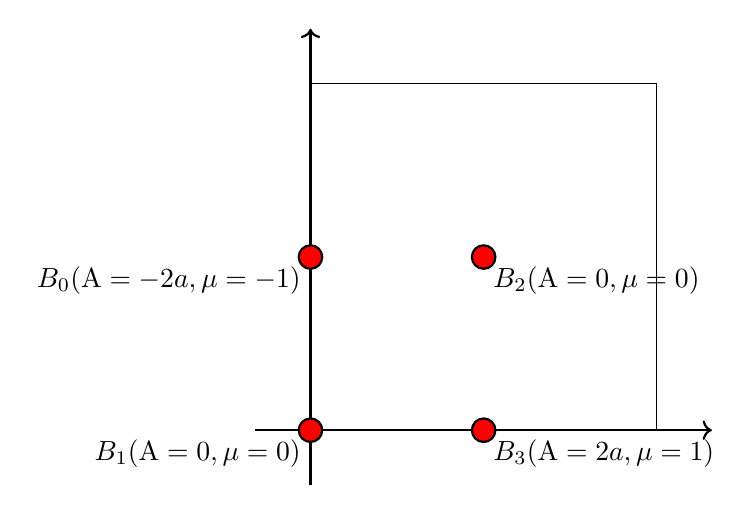
\begin{tikzpicture}[scale=0.7, vertex/.style={draw,circle,thick,fill=red,inner sep=3pt}]
\draw[->,thick] (-1,0) -- (2*pi+1,0);
\draw[->,thick] (0,-1) -- (0,2*pi+1);
\draw (0,0) rectangle (2*pi,2*pi);

\draw (0,0) node[vertex] {} node[below left] {$B_1 (\AA = 0, \mu = 0)$};
\draw (0,pi) node[vertex] {} node[below left] {$B_0 (\AA = -2a, \mu = -1)$};
\draw (pi,0) node[vertex] {} node[below right] {$B_3 (\AA = 2a, \mu = 1)$};
\draw (pi,pi) node[vertex] {} node[below right] {$B_2 (\AA = 0, \mu = 0)$};
\end{tikzpicture}
\caption{The periodic orbits of $H_1$ and their actions and Maslov indices}
\end{figure}

Consequently, the vector spaces of the Floer complex are given by
\begin{equation}
\begin{gathered}
\CF_{-1}^\lambda(H_1) = \begin{cases}
0, & \lambda \leq -2a,\\
\braket{B_0} & \lambda > -2a,
\end{cases}
\\
\CF_{0}^\lambda(H_1) = \begin{cases}
0, & \lambda \leq 0,\\
\braket{B_1,B_2} & \lambda > 0,
\end{cases}
\\
\CF_{1}^\lambda(H_1) = \begin{cases}
0, & \lambda \leq \leq 2a,\\
\braket{B_3} & \lambda  > 2a.
\end{cases}
\end{gathered}
\end{equation}

This information can be sumarily represented via the following barcode.
\begin{figure}[H]
\centering
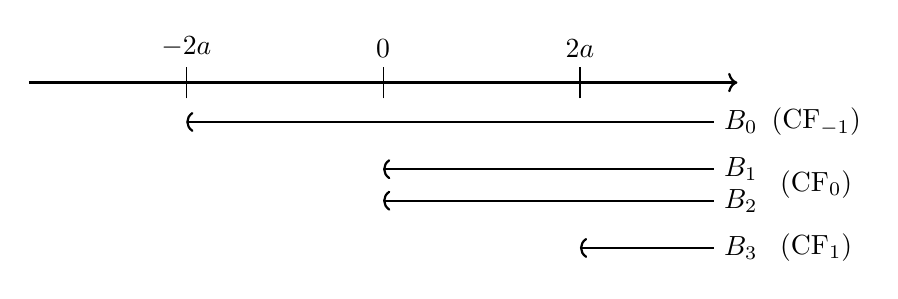
\begin{tikzpicture}
\draw[->,thick] (-4.500,0.000)--(4.500,0.000);
\draw[] (0.000,-0.200)--(0.000,0.200) node[above] {0};
\draw[] (2.500,-0.200)--(2.500,0.200) node[above] {$2a$};
\draw[] (-2.500,-0.200)--(-2.500,0.200) node[above] {$-2a$};
\draw[(-,thick] (-2.500,-0.500)--(4.200,-0.500) node[right] {$B_0$};
\node[] at (5.500,-0.500) {$(\CF_{-1})$};
\draw[(-,thick] (0.000,-1.100)--(4.200,-1.100) node[right] {$B_1$};
\draw[(-,thick] (0.000,-1.500)--(4.200,-1.500) node[right] {$B_2$};
\node[] at (5.500,-1.300) {$(\CF_0)$};
\draw[(-,thick] (2.500,-2.100)--(4.200,-2.100) node[right] {$B_3$};
\node[] at (5.500,-2.100) {$(\CF_1)$};
\end{tikzpicture}
\caption{The barcode of the filtered Floer complex of $H_1$}
\end{figure}
\end{prop}

All that remains is to compute the boundary maps $\partial$. We will show that they are null, by exploiting symmetries of the space $M$ and the Hamiltonian $H_1$.

\subsection{Symmetries}

We begin by recalling the definition of $\partial(b)$, where $b$ is a periodic orbit of $H_1$. First, one must compute the Maslov index $\mu(b)$. Then, $\partial(b)$ will be of the form
\begin{equation}
\partial(b) = \sum n(b,c) c,
\end{equation}
where the sum is taken over orbits $c$ whose Maslov index is $\mu(c) = \mu(b)-1$. The numbers $n(b,c)$ are computed by counting how many pseudo-holomorphic curves connect $b$ and $c$. A pseudo-holomorphic curve is a $C^\infty$ function $(x(t,s), y(t,s))$, $t \in \R / T$, $s \in \R$, satisfying
\begin{equation}
\begin{cases}
\displaystyle \diffp x s - \diffp y t = \diffp H x,\\[1em]
\displaystyle \diffp y x + \diffp x t = \diffp H y.
\end{cases}
\end{equation}

We say that such a curve $(x,y)$ connects the periodic orbits $b$ and $c$ if the following limits hold in the $C^\infty$ sense
\begin{equation}
\lim_{s \to -\infty} (x,y)(t,s) = b(t), \; \lim_{s \to \infty} (x,y)(t,s) = c(t).
\end{equation}

The set of such solutions, modulo translation of $s$, is denoted $\moduli(b,c)$.

Now, we are only interested in the number of said curves modulo 2, so if we find any symmetries in $\moduli(b,c)$ in the form of an involution $F \colon \moduli(b,c) \to \moduli(b,c)$ we will only need to examine solutions which are symmetrical, i.e. $F(u) = u$. In our case, such involutions will come from well-chosen changes of variable.
% !TeX root = Thesis.tex
\chapter{The Barcode of Another Non-Autonomous Hamiltonian}
\label{chap:secondexample}

Let us now consider the Hamiltonian diffeomorphism $\phi^2$, where $\phi$ is the diffeomorphism considered in the previous chapter, i.e.
\begin{equation}
\phi(x,y) = ( x + a \sin(y + a \sin(x)), y + a \sin(x)).
\end{equation}

The Hamiltonian diffeomorphism $\phi$ is the time $2a$ flow of the Hamiltonian $H_1$ (see \eqref{h1def}), defined in $\interval 0 {2a}$. Consequently, $\phi^2$ is the time $4a$ flow of the same Hamiltonian, extended by periodicity to the interval $\interval 0 {2a}$.

In chapter \ref{chap:firstexample}, we saw that the behavior of the barcode of $\phi$ did not qualitatively depend on the value of $a > 0$. We will see that for $\phi^2$ this does not occur, and the barcode goes through phase changes at $a = 2$ and $a = \pi$. It is very likely that the behavior becomes increasingly complicated, going through more changes, as $a \to \infty$, but here we restrict our attention to $0 < a < \pi$.

We begin by computing the contractible $2a$-periodic orbits of $H_1$ in the torus, i.e. the solutions of $\tilde \phi^2(x,y) = (x,y)$ in $\R^2$, where $\tilde \phi$ is the flow of $H_0 \circ \pi$ (see corollary \ref{cor:liftham}).

\section{The Contractible Periodic Orbits}

\begin{prop}\label{prop:orbitsphi2}
If $a \leq 2$, the solutions to the equation $\tilde \phi^2(x,y) = (x,y)$ coincide with the solutions of $\phi(x,y) = (x,y)$, i.e. $(x,y) \in \pi \Z \times \pi \Z$.

If $2 < a < \pi$, there are four new solutions modulo $2\pi$. Let $(x_0, y_0)$ be the unique solution in $\ointerval 0 \pi \times \ointerval 0 \pi$. Then, the other three solutions are given by rotations of this solution about the origin, i.e.
\begin{equation}
(x_0, y_0), (-y_0, x_0), (-x_0, -y_0), \text{ and } (y_0, -x_0).
\end{equation}

Furthermore, $y_0 = \pi - x_0$, and $x_0$ is defined as the unique positive fixed point of $x \mapsto \frac a 2 \sin(x)$.
\end{prop}

\begin{proof}
We begin by writing out the equation $\tilde\phi^2(x,y) = (x,y)$ in full:
\begin{equation}\label{phi2id1}
\begin{gathered}
\begin{cases}
x + a \sin(y + a \sin(x)) + a \sin(y_2) = x,\\
y_2 = y,
\end{cases}\\
\text{Where $y_2 = y + a \sin(x) + a \sin(x + a \sin(y + a \sin(x)))$.}
\end{gathered}
\end{equation}

A few elementary computations will show that, for $a > 0$, equation \eqref{phi2id1} is equivalent to
\begin{equation}\label{phi2id2}
\begin{cases}
\sin(y + a \sin(x)) + \sin(y) = 0,\\
\sin(x - a \sin(y)) + \sin(x) = 0.
\end{cases}
\end{equation}

Now, recall that an equation of the form $\sin(A) = - \sin(B)$ has two types of solutions:
\begin{equation}
\begin{aligned}
A &= - B + 2 k \pi, \; k \in \Z && \text{(Type 1)}\\
A &= \pi + B + 2 k \pi, \; k \in \Z && \text{(Type 2).}
\end{aligned}
\end{equation}

The restriction $a < \pi$ implies that neither of the equations in \eqref{phi2id2} has solutions of type 2. For example, a type 2 solution of the first equation would satisfy
\begin{equation}
y + a \sin(x) = \pi + y + 2 k \pi \iff a \sin(x) = \pi + 2 k \pi,
\end{equation}
which is impossible because the left-hand side is always less than $\pi$ in absolute value, while the right-hand side is always greater than or equal to $\pi$ in absolute value.

Therefore, the system \eqref{phi2id2} reduces to
\begin{equation}
\begin{cases}
y = - \frac a 2 \sin(x) + k_1 \pi,\\
x = \frac a 2 \sin(y) + k_2 \pi.
\end{cases}
\end{equation}

Modulo $2\pi$, there are only two cases, $(k_1, k_2) \in \{0,1\} \times \{0,1\}$.

We begin by showing that if $k_1 = k_2$ then there are only the trivial solutions $x = y = k_1 \pi$.

\begin{lemma}
For $k = 0, 1$ and $0 < a < \pi$, the system of equations
\begin{equation}
\begin{cases}
y = - \frac a 2 \sin(x) + k \pi,\\
x = \frac a 2 \sin(y) + k \pi,
\end{cases}
\end{equation}
has only the trivial solution $x = y = k \pi$.
\end{lemma}

\begin{lemmaproof}
It suffices to consider the case $k = 0$, as the other case can be reduced to this one via a change of variables. Suppose then that
\begin{equation}
\begin{cases}
y = - \frac a 2 \sin(x),\\
x = \frac a 2 \sin(y).
\end{cases}
\end{equation}

In this case, $x = - \frac a 2 \sin\left(\frac a 2 \sin(x)\right)$. Such a solution must satisfy $\abs x \leq \frac a 2 < \frac \pi 2$, and therefore the sign of $\sin(x)$ coincides with the sign of $x$. For the same reason $(\abs{\frac a 2 \sin(x)} \leq \frac a 2 < \frac \pi 2)$, the sign of $\sin\left(\frac a 2 \sin(x) \right)$ coincides with the sign of $\frac a2 \sin(x)$, which coincides with the sign of $x$. Unless $x=0$, this is an obvious contradiction.
\end{lemmaproof}

We now handle the case $k_1 \neq k_2$.

\begin{lemma}
For $k = 0, 1$ and $0 < a \leq 2$, the system of equations
\begin{equation}\label{phi2id3}
\begin{cases}
y = - \frac a 2 \sin(x) + k \pi,\\
x = \frac a 2 \sin(y) + (1-k) \pi,
\end{cases}
\end{equation}
has only the trivial solution $x = y = k \pi$.

On the other hand, if $2 < a < \pi$, there exist two new solutions for each value of $k$. The solutions $(x,y)$ to the case $k=0$ are in bijection with the solutions to the case $k=1$, via the map
\begin{equation}
(x,y) \mapsto (y, 2\pi - x).
\end{equation}

Furthermore, if $(x_0, y_0)$ is the unique solution to the $k=0$ case with $x_0 > 0$, we have $y_0 = \pi - x_0$. Finally, the three solutions to the $k = 0$ case are $(-x_0, -y_0)$, $(0,0)$ and $(x_0, y_0)$.
\end{lemma}

\begin{lemmaproof}
The bijection between the solutions of the $k=0$ and $k=1$ cases holds regardless of the value of $a$, so both for $0<a\leq 2$ and for $2<a<\pi$ it suffices to verify the case $k=1$.

To find solutions of \eqref{phi2id3} for $k=1$, consider the map
\begin{equation}
\eta(x) = \frac a 2 \sin(x).
\end{equation}

Then, solutions of \eqref{phi2id3} are in one-to-one correspondence with fixed points of $\eta^2 = \eta \circ \eta$, so it suffices to consider that problem instead. Furthermore, since $\eta$ is odd, and consequently so is $\eta^2$, it suffices to look for positive solutions, which must obviously be in the interval $\linterval 0 {\frac a 2}$. Here are some facts about $\eta$ and $\eta^2$, which can be deduced by elementary calculus.
\begin{itemize}
\item The derivatives of $\eta$ and $\eta^2$ at zero are given by $\frac a 2$ and $\left( \frac a 2 \right)^2$ respectively,
\item Both of these functions are concave in $\interval 0 {\frac a 2}$, because their second derivative is negative (strictly except at zero),
\item Both of these functions are increasing in the interval $\interval 0 {\frac a 2}$. This uses the fact that $a < \pi$.	
\end{itemize}

The case $a < 2$ is now easy to solve, as in this event the derivative of $\eta^2(x) - x$ is negative at zero and decreasing in $\interval 0 {\frac a 2}$. Therefore, $\eta^2(x) - x$ is a decreasing function, and since it takes the value $0$ at $x = 0$, it cannot vanish again in $\interval0{\frac a 2}$.

The case $a = 2$ is similar, though not as direct because the derivative of $\eta^2(x) - x$ at zero is now zero, instead of negative. However, by concavity, this function is still strictly decreasing in $\interval 0 {\frac a 2}$ and the same argument goes through.

Finally, we consider $2 < a < \pi$. In this case, the derivative of $\eta(x) - x$ is positive at zero, and therefore, for small enough values of $x$, $\eta(x) > x$. On the other hand, since $\abs{\eta(x)} \leq \frac a 2$ for all $x$, obviously $\eta(\frac a 2) \leq \frac a 2$. Therefore, by continuity, we have established the existence of a fixed point of $\eta$ in $\linterval 0 {\frac a 2}$, and consequently of a fixed point of $\eta^2$.

We now show that such a fixed point is unique. Since $\eta^2(x)$ is concave in the interval, so is $\eta^2(x) - x$. It is a known fact that a strictly concave function on an interval attains each value at most twice, and so in particular has at most two roots. One of the roots is $x = 0$, and the other is the root which we have proven exists. We call this root $x_0$. To it we associate a solution $(x_0, y_0)$ of \eqref{phi2id3}, satisfying $y_0 = \pi - \eta(x_0)$ and $x_0 = \eta(y_0)$. Note that we have constructed $x_0$ as a fixed point of $\eta$, hence $\eta(x_0) = x_0$ and therefore that $y_0 = \pi - x_0$. This completes the proof of the lemma...
\end{lemmaproof}
...and therefore of the proposition.
\end{proof}

Now that we have computed the contractible periodic orbits of $H_1$ we may label them. We have already labeled the fixed points of $\phi$ as $B_0, \dots, B_3$. In the case $a > 2$, we have four new periodic orbits, which come in pairs, because they stem from pairs of points $p_1, p_2$ satisfying $\phi(p_1) = p_2$ and $\phi(p_2) = p_1$.

Let $A_0$ refer to the orbit starting at $(x_0, y_0)$, where $(x_0, y_0)$ is as in proposition \ref{prop:orbitsphi2}, and let $A_1$ refer to the orbit starting at $(-x_0, -y_0)$. Likewise, let $C_0$ be the orbit starting at $(-y_0, x_0)$ and $C_1$ be the orbit starting at $(y_0, -x_0)$. For convenience, these labels are represented in figure \ref{orbitsh12}.

In what follows, to avoid needlessly reminding of ourselves of the conditions on $a$, we adopt the convention: \emph{$a$ is always in $\ointerval 0 \pi \setminus \{2\}$, and whenever we refer to the orbits $A_i$ and $C_i$ it should be tacitly assumed that $a > 2$.}

\begin{figure}
\centering
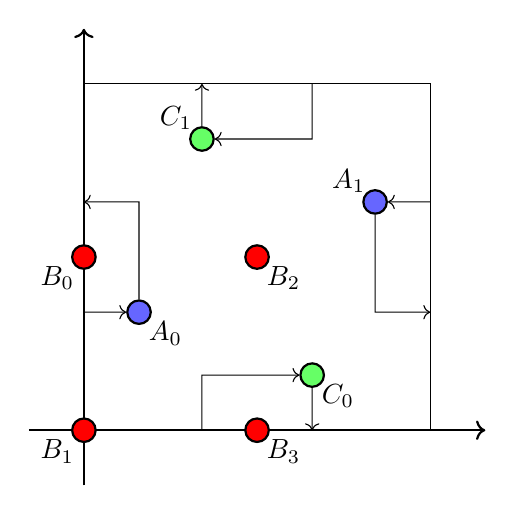
\begin{tikzpicture}[scale=0.7, vertex/.style={draw,circle,thick,fill=red,inner sep=3pt}]
\draw[->,thick] (-1,0) -- (2*pi+1,0);
\draw[->,thick] (0,-1) -- (0,2*pi+1);
\draw (0,0) rectangle (2*pi,2*pi);

\draw (0,0) node[vertex] {} node[below left] {$B_1$};
\draw (0,pi) node[vertex] {} node[below left] {$B_0$};
\draw (pi,0) node[vertex] {} node[below right] {$B_3$};
\draw (pi,pi) node[vertex] {} node[below right] {$B_2$};

\node[vertex,fill=blue!60] (A0) at (1,pi-1) {};
\node[vertex,fill=blue!60] (A1) at (2*pi-1,pi+1) {};
\draw[->] (0,pi-1) -- (A0);
\draw[->] (A0) node[below right] {$A_0$} -- (1,pi+1) -- (0,pi+1);
\draw[->] (2*pi,pi+1) -- (A1);
\draw[->] (A1) node[above left] {$A_1$} -- (2*pi-1,pi-1) -- (2*pi,pi-1);

\node[vertex,fill=green!60] (C0) at (pi+1,1) {};
\node[vertex,fill=green!60] (C1) at (pi-1,2*pi-1) {};
\draw[->] (C0) -- (pi+1,0);
\draw[->] (pi-1,0) -- (pi-1,1) -- (C0) node[below right] {$C_0$};
\draw[->] (C1) -- (pi-1,2*pi);
\draw[->] (pi+1,2*pi) -- (pi+1,2*pi-1) -- (C1) node[above left] {$C_1$};
\end{tikzpicture}
\caption{The contractible $4a$-periodic orbits of $H_1$ ($a > 2$), labeled. The label of an orbit is next to its starting point. For the non-constant orbits, the arrow represents the time-$2a$ flow.}
\label{orbitsh12}
\end{figure}

\section{The Actions}

We now compute the actions of the orbits $A_0$, $A_1$, $B_0, \dots, B_3, C_0$ and $C_1$.

We begin with the constant orbits $B_i$. By a similar argument as the one done for the case of the Hamiltonian diffeomorphism $\phi$, the action of these orbits is simply the integral of $H_1$ at these points, which is given by $2a(\cos(y) - \cos(x))$. This concludes the computation of the action spectrum for $a < 2$.

Let us now inspect the orbits $A_i$ and $C_i$. The paths taken by these orbits are squares, and therefore we may consider the extension of the orbits to the disk in the definition of the action functional to be a diffeomorphism between the interior of the disk and these squares. Furthermore, since the symplectic form $\omega$ is the area form on the torus, it pulls back to the area form on the square. Consequently, the $- \int_D \omega$ term in the action functional will be equal to the area of the square or its symmetric, depending on the orientation of the border: In the counterclockwise case ($A_0$, $A_1$) the orientation is positive, yielding a negative contribution, while in the clockwise case ($C_0$, $C_1$) it is negative, yielding a positive contribution. Finally, the area of these squares, in absolute value, is equal to their side squared, i.e. $(2x_0)^2 = 4x_0^2$.

Now we inspect the $\int H_1$ term in the action functional applied to these orbits. For the sake of concreteness, we will compute it for $A_0$, but the same argument goes for the other three orbits.

The orbit $A_0$ can be divided into four (reparametrized) linear segments. For example, the first segment goes from $(x_0, y_0)$ to $(x_0, y_0 + 2a \sin(x_0)) = (x_0, \pi + x_0)$. Over this segment, the Hamiltonian $H_1$ takes the value $- \varphi(t) \cos(x_0)$ at time $t$, (see definition of $H_1$ at \eqref{h1def}) and integrating we obtain a contribution of $- a \cos(x_0)$ to $\int H_1$. It is easy to compute the contributions of the four other line segments: they are all also equal to $- a \cos(x_0)$, and so we conclude
\begin{equation}
\AA(A_0) = - 4 x_0^2 - 4 a \cos(x_0).
\end{equation}

This value coincides with $\AA(A_1)$, and furthermore
\begin{equation}
\AA(C_0) = \AA(C_1) = - \AA(A_0).
\end{equation}

As a last remark, we prove a simple inequality regarding $\AA(A_0)$, so that we can place the actions we have calculated so far on a line.

\begin{prop}\label{prop:ineq4beta}
Let $2 < a < \pi$ and $x_0$ be as in proposition \ref{prop:orbitsphi2}. Then, we have the inequality
\begin{equation}
0 < 4 x_0^2 + 4 a \cos(x_0) < 4a.
\end{equation}
\end{prop}

\begin{proof}
Since $0 < x_0 < \pi$, it should be obvious that $4 x_0^2 + 4 a \cos(x_0) > 0$, as it is a sum of two positive terms. Therefore, we turn to proving the other inequality.

Recall that $x_0$ satisfies the equality $x_0 = \frac a 2 \sin(x_0)$. Consequently, $4 x_0^2 = a^2 \sin^2 (x_0) = a^2 - a^2 \cos^2(x_0)$. Therefore,
\begin{equation}
4 x_0^2 + 4 a \cos(x_0) = a^2 + 4 a \cos(x_0) - a^2 \cos^2(x_0).
\end{equation}

Therefore, to show that $4 x_0^2 + a \cos(x_0) < 4a$ it suffices to show
\begin{equation}\label{eq:ineq4beta}
\begin{aligned}
&& a^2 + 4 a \cos(x_0) - a^2 \cos^2(x_0) &< 4a\\
\iff&& 4 (\cos(x_0)-1) + a(1 - \cos^2(x_0)) &< 0\\
\iff&& (\cos(x_0) - 1)(4 - a(1 + \cos(x_0))) &< 0\\
\iff&& 4 - a(1+ \cos(x_0)) &> 0\\
\iff&& a + a \cos(x_0) &< 4.
\end{aligned}
\end{equation}

The proof of this last inequality is somewhat involved. We begin by writing $a$ as a function of $x_0$, as
\begin{equation}
a = \frac{2 x_0}{\sin(x_0)}.
\end{equation}

Therefore, we intend to show that, for $x_0$ in, say, $\interval 0 {\frac \pi 2}$, the expression $\frac{x_0}{\sin(x_0)}(1 + \cos(x_0))$ is always less than 2. To this effect, we study the function
\begin{equation}
f(t) = \frac{t}{\sin(t)}(1 + \cos(t)).
\end{equation}

Laborious but straightforward computations will show that the derivative of $f$ is given by
\begin{equation}
f'(t) = - \frac{t - \sin(t)}{1 - \cos(t)}.
\end{equation}

Evidently, for $t > 0$, $f'(t) < 0$ where defined. Consequently, $f$ is a strictly decreasing function. Since $\lim_{t \to 0^+} f(t) = 2$, we obtain that $f(t) < 2$ for $t \in \ointerval 0 {\frac \pi 2}$, which completes the proof.
\end{proof}

We can now place the actions of the orbits on the real line, see figure \ref{actionsh12}.

\begin{figure}
\centering
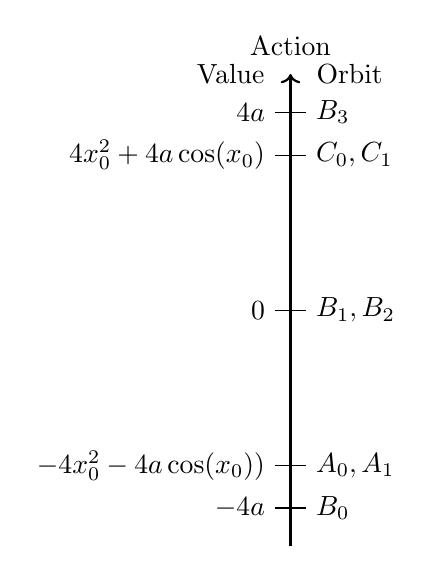
\begin{tikzpicture}[scale=0.2, tick/.style={left=0.2cm}, value/.style={right=0.2cm}]
\draw[->,thick] (0, -15) -- (0,15) node[above=0.1cm] {Action} node[tick] {Value} node[value]{Orbit};

\foreach \x in {-12.56,-9.85,0,9.85,12.56}
\draw (-1, \x) -- (1,\x);

\draw (0,-12.56) node[tick] {$-4a$} node[value] {$B_0$};
\draw (0,-9.85) node[tick] {$-4x_0^2 - 4 a \cos(x_0))$} node[value] {$A_0, A_1$};
\draw (0,0) node[tick] {$0$} node[value] {$B_1, B_2$};
\draw (0,9.85) node[tick] {$4x_0^2 + 4 a \cos(x_0)$} node[value] {$C_0, C_1$};
\draw (0,12.56) node[tick] {$4a$} node[value]  {$B_3$};


\end{tikzpicture}
\caption{The actions of the contractible periodic orbits of $H_1$ in time $4a$. The figure is to scale, with $a = 3.14$. As $a$ gets closer to $2$, the value of $4x_0^2 + 4a \cos(x_0)$ gets closer to $4a$.}
\label{actionsh12}
\end{figure}

\section{The Maslov Indices}

We will now use corollary \ref{calcmaslov1} to compute the Maslov indices of the contractible orbits calculated above.

We begin with the orbits $B_0, \dots, B_3$, which are present for all $a > 0$. On these, the derivative can be calculated in a way similar to the computations in page \pageref{rectpath1}. Using the same notation as therein to represent piecewise rectilinear paths, the derivative matrix $A(t)$ at each $B_i$ is given by
\begin{equation}
\begin{multlined}
A(t):
\begin{bmatrix}
1 & 0\\
0 & 1
\end{bmatrix}
\to
\begin{bmatrix}
1 & 0\\
\pm_1 a & 1
\end{bmatrix}
\to
\begin{bmatrix}
1 \pm_1 \pm_2 a^2 &  \pm_2 a\\
\pm_1 a & 1
\end{bmatrix}\\
\to
\begin{bmatrix}
1 \pm_1 \pm_2 a^2 &  \pm_2 a\\
\pm_1 2a \pm_2 a^3 & 1 \pm_1 \pm_2 a^2
\end{bmatrix}
\to
\begin{bmatrix}
1 \pm_1 \pm_2 3 a^2 + a^4 &  \pm_2 2 a \pm_1 a^3\\
\pm_1 2a \pm_2 a^3 & 1 \pm_1 \pm_2 a^2
\end{bmatrix},
\end{multlined}
\end{equation}
where $\pm_1 1 = \cos(x)$ and $\pm_2 1 = \cos(y)$. We may now compute the trace of $A(t)$:
\begin{equation}
\trace A(t): 2 \to 2 \to 2 \pm_1 \pm_2 a^2 \to 2 \pm_1 \pm_2 2 a^2 \to 2 \pm_1 \pm_2 4 a^2 + a^4.
\end{equation}

We may remove the superfluous middle node, obtaining the equivalent representation
\begin{equation}\label{tracebi}
\trace A(t): 2 \to 2 \to 2 \pm_1 \pm_2 2 a^2 \to 2 \pm_1 \pm_2 4 a^2 + a^4.
\end{equation}

\begin{prop}
The Maslov indices of $B_1$ and $B_2$ are null.
\end{prop}

\begin{proof}
In this case, using the notation of equation \eqref{tracebi}, $\pm_1 = \pm_2$ and therefore the trace is always greater than or equal to two. Per corollary \ref{calcmaslov1}, this implies that the Maslov index is null.
\end{proof}

\begin{prop}
If $a < 2$, the Maslov indices of $B_0$ and $B_3$ are $-1$ and $1$ respectively. If $a > 2$, they are $-2$ and $2$.
\end{prop}

\begin{proof}
In this case, $\pm_1 \neq \pm_2$, and therefore the trace follows the path
\begin{equation}
\trace A(t) : 2 \to 2 \to 2 - 2a^2 \to 2 - 4a^2 + a^4.
\end{equation}

If $a<2$ then the trace starts at $2$, decreases, and doesn't reach $2$ again, as $2 - 4a^2 + a^4 = 2 - a^2 (a^2 - 4) < 2$. Therefore, we consider the partition $a_0 = 0$, $b_0 = 2a$, which is in the conditions of corollary \ref{calcmaslov1}, and so, for $a<2$,
\begin{equation}
\mu(A(t)) = \sign(A(2a)_{12}) = \sign(\pm_2 a) = \pm_2 1,
\end{equation}
which is what we wanted to prove.

\smallskip

We now consider the case $a > 2$. In this case the trace starts at 2, decreases to less than $-2$ and goes back up to more than 2 again. Therefore, our partition will now be of the form $a_0 < b_0 < a_1 < b_1$.

We set $a_0 = 0$ and $a_1 = 2a$. We define $b_0 = a(1+\varepsilon)$ for some small $\varepsilon$, in which case $\sign(A(b_0)_{12}) = \pm_2 1$.

The choice for $b_1$ is a bit trickier. We define $b_1$ in order to make the trace of $A(t)$ equal to zero, i.e., $b_1 = a(3 + t_0)$, where $t_0$ satisfies
\begin{equation}
2 - 2a^2 + (-2a^2 + a^4)t_0 = 0 \iff t_0 = \frac{2a^2 - 2}{a^4 - 2a^2}.
\end{equation}
Note: We don't need to verify that this expression is in $\interval 0 1$. It must be, because $t_0$ was defined as the root of an affine function, which is known to be less than $-2$ at zero and greater than $2$ at one.

We can now compute $A(b_1)_{12}$ explicitly as
\begin{equation}
\pm_2 a \pm_2 (a - a^3) t_0 = \mp_2 \frac{2 + a^2(a^2 - 2)}{a(a^2 - 2)}.
\end{equation}

Given that $a^2 > 4 > 2$, the right-hand side has sign equal to $\mp_2$. In other words, $\sign(A(b_1)_{12}) = \mp_2 1$, and so, applying corollary \ref{calcmaslov1} we obtain
\begin{equation}
\mu(A(t)) = \pm_2 2.
\end{equation}

This completes the proof.
\end{proof}

We now turn to computing the Maslov indices of $A_1$, $A_2$, $C_1$ and $C_2$. To this effect, we begin by computing $(\dl \phi_t)_{(x_0,y_0)}$, in order to calculate the Maslov index of $A_1$.

Recall equation \eqref{eq:rectpath}, which describes the path $A(t) = (\dl \phi_t)_{(x,y)}$ up to time $2a$ (using the Hamiltonian $H_0$)
\begin{equation}\label{eq:rectpath2}
A(t) :
\begin{bmatrix}
1 & 0\\
0 & 1
\end{bmatrix}
\to
\begin{bmatrix}
1 & 0\\
a \cos(x) & 1
\end{bmatrix}
\to
\begin{bmatrix}
\scalebox{0.7}{$1+ a^2 \cos(y+a \sin(x)) \cos(x)$} &  a \cos(y)\\
a \cos(x) & 1
\end{bmatrix}.
\end{equation}

We plug in $(x,y) = (x_0, y_0)$. To simplify the expressions, we set $\beta = a \cos(x_0)$, to obtain
\begin{equation}
A(t) :
\begin{bmatrix}
1 & 0\\
0 & 1
\end{bmatrix}
\to
\begin{bmatrix}
1 & 0\\
\beta & 1
\end{bmatrix}
\to
\begin{bmatrix}
1 - \beta^2 &  -\beta \\
\beta & 1
\end{bmatrix}, t \in \interval 0 {2a}.
\end{equation}

Note that if we set $(x,y) = (-x_0, -y_0)$ we obtain the same expression. Furthermore, we have seen that $\phi(x_0, y_0) = (-x_0, -y_0)$, so that 1. the expression for $A(t)$ is the same if we start at $(-x_0, -y_0)$ and 2. by the chain rule we may write
\begin{equation}
A(2a + t) = A(2a) A(t), t \in \interval 0 {2a}.
\end{equation}

Therefore, the expression for $A(t)$ for $t \in \interval 0 {4a}$, associated to the paths $A_0$ and $A_1$, is given by
\begin{equation}
\begin{multlined}
A(t) :
\begin{bmatrix}
1 & 0\\
0 & 1
\end{bmatrix}
\to
\begin{bmatrix}
1 & 0\\
\beta & 1
\end{bmatrix}
\to
\begin{bmatrix}
1 - \beta^2 &  -\beta \\
\beta & 1
\end{bmatrix}\\
\to
\begin{bmatrix}
1 - \beta^2 &  -\beta \\
2 \beta - \beta^3 & 1 - \beta^2
\end{bmatrix}
\to
\begin{bmatrix}
1 - 3 \beta^2 + \beta^4 &  -2 \beta + \beta^3 \\
2 \beta - \beta^3 & 1 - \beta^2
\end{bmatrix}.
\end{multlined}
\end{equation}

Therefore, the trace of $A(t)$ follows the path
\begin{equation}
\trace A(t) : 2 \to 2 \to 2 - 2\beta^2 \to 2 - 4 \beta^2 + \beta^4,
\end{equation}
where the nodes are respectively at $0$, $a$, $3a$ and $4a$. The following proposition helps us describe qualitatively the behavior of the trace.

\begin{prop}
Using the notation $\beta = a \cos(x_0)$, we have the inequalities
\begin{align}
\label{beta1} 0 < \beta^2 &< 4\\
\label{beta2} -2 < 2 - \beta^2 &< 2,\\
\label{beta3} 2-2\beta^2 &< 2\\
\label{beta4} 2 - 4 \beta^2 + \beta^4 &< 2.
\end{align}
\end{prop}

\begin{proof}
We begin by proving \eqref{beta1}. The inequality $\beta^2 > 0$ is obvious from the fact that $\beta \neq 0$, as $0 < x_0 < \frac\pi2$. For the inequality $\beta^2 < 4$ we use the fact, which we proved in the middle of proving proposition \ref{prop:ineq4beta} (see equation \eqref{eq:ineq4beta}) that
\begin{equation}
\beta < 4 - a,
\end{equation}
and using the fact that $a > 2$ we immediately obtain $\beta < 2$ and hence $\beta^2 < 4$. This proves \eqref{beta1}.

Inequality \eqref{beta2} is obvious from \eqref{beta1}, and \eqref{beta3} is also obvious using $2 - 2 \beta^2 < 2 - \beta^2$. Finally, to prove \eqref{beta4} we use the factorization
\begin{equation}
2 - 4 \beta^2 + \beta^4 = 2 + \beta^2 (\beta^2 - 4).
\end{equation}

Since $\beta^2$ is positive and $\beta^2 - 4$ is negative, we obtain the desired inequality.
\end{proof}

\begin{corollary}
Let $A(t)$ be the matrix path given by the derivative of the flow of $H_0$ in the orbits $A_0$ and $A_1$. Then, the trace of $A(t)$ starts at 2, followed by a decrease, after which it always stays strictly below 2 (by \eqref{beta3} and \eqref{beta4}). Furthermore, $\trace A(2a) = 2 - \beta^2$ is in $\ointerval{-2}2$ (by \eqref{beta2}).
\end{corollary}

We are now able to compute the Maslov index of $A(t)$, and consequently the Maslov indices of the orbits $A_0$ and $A_1$. We apply corollary \ref{calcmaslov1}, using the partition $a_0 = 0$ and $b_0 = 2a$. The conditions of this corollary are verified, and hence
\begin{equation}
\mu(A(t)) = \sign(-\beta) = -1,
\end{equation}
because $\beta$ is positive. Therefore,

\begin{prop}
The Maslov index of $A_0$ and $A_1$ is $-1$.
\end{prop}

The same computations apply almost without change for the orbits $C_0$ and $C_1$. The main difference is that $A(t)$ now becomes
\begin{equation}
\begin{multlined}
A(t) :
\begin{bmatrix}
1 & 0\\
0 & 1
\end{bmatrix}
\to
\begin{bmatrix}
1 & 0\\
-\beta & 1
\end{bmatrix}
\to
\begin{bmatrix}
1 - \beta^2 &  \beta \\
-\beta & 1
\end{bmatrix}\\
\to
\begin{bmatrix}
1 - \beta^2 &  \beta \\
-2 \beta + \beta^3 & 1 - \beta^2
\end{bmatrix}
\to
\begin{bmatrix}
1 - 3 \beta^2 + \beta^4 &  2 \beta - \beta^3 \\
-2 \beta + \beta^3 & 1 - \beta^2
\end{bmatrix},
\end{multlined}
\end{equation}
that is, the signs of the non-diagonal elements have been swapped. This preserves the trace and so the application of corollary \ref{calcmaslov1}, except that the term $\sign(-\beta)$ now becomes $\sign(\beta) = 1$. Consequently,

\begin{prop}
The Maslov index of $C_0$ and $C_1$ is 1.
\end{prop}

\begin{corollary}
The vector spaces of the filtered Floer complex of $H_1$ in time $4a$ are given by the following labeled barcodes. Figure \ref{bch1lt2} denotes the case where $0<a<2$ and figure \ref{bch1gt2} denotes the case $2<a<\pi$.

\begin{figure}[H]
\centering
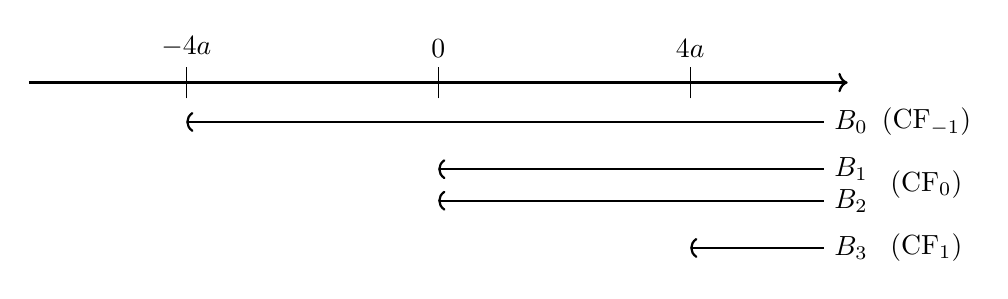
\begin{tikzpicture}
\draw[->,thick] (-5.200,0.000)--(5.200,0.000);
\draw[] (0.000,-0.200)--(0.000,0.200) node[above] {0};
\draw[] (-3.200,-0.200)--(-3.200,0.200) node[above] {$-4a$};
\draw[] (3.200,-0.200)--(3.200,0.200) node[above] {$4a$};
\draw[(-,thick] (-3.200,-0.500)--(4.900,-0.500) node[right] {$B_0$};
\node[] at (6.200,-0.500) {$(\CF_{-1})$};
\draw[(-,thick] (0.000,-1.100)--(4.900,-1.100) node[right] {$B_1$};
\draw[(-,thick] (0.000,-1.500)--(4.900,-1.500) node[right] {$B_2$};
\node[] at (6.200,-1.300) {$(\CF_0)$};
\draw[(-,thick] (3.200,-2.100)--(4.900,-2.100) node[right] {$B_3$};
\node[] at (6.200,-2.100) {$(\CF_{1})$};
\end{tikzpicture}
\caption{The barcode of the filtered Floer complex of $H_1$ in time $4a$, for $0<a<2$}\label{bch1lt2}
\end{figure}

\begin{figure}[H]
\centering
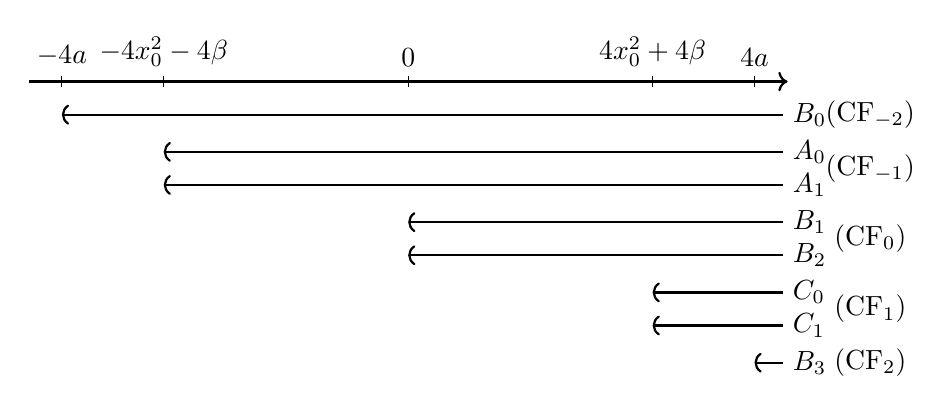
\begin{tikzpicture}[scale=0.35]
\draw[->,thick] (-13.766,0.000)--(13.766,0.000);
\draw[] (0.000,-0.200)--(0.000,0.200) node[above] {0};
\draw[] (-12.566,-0.200)--(-12.566,0.200) node[above] {$-4a$};
\draw[] (12.566,-0.200)--(12.566,0.200) node[above] {$4a$};
\draw[] (-8.870,-0.200)--(-8.870,0.200) node[above] {$-4 x_0^2 - 4 \beta$};
\draw[] (8.870,-0.200)--(8.870,0.200) node[above] {$4 x_0^2 + 4 \beta$};
\draw[(-,thick] (-12.566,-1.200)--(13.586,-1.200) node[right] {$B_0$};
\node[] at (16.766,-1.200) {$(\CF_{-2})$};
\draw[(-,thick] (-8.870,-2.550)--(13.586,-2.550) node[right] {$A_0$};
\draw[(-,thick] (-8.870,-3.750)--(13.586,-3.750) node[right] {$A_1$};
\node[] at (16.766,-3.150) {$(\CF_{-1})$};
\draw[(-,thick] (0.000,-5.100)--(13.586,-5.100) node[right] {$B_1$};
\draw[(-,thick] (0.000,-6.300)--(13.586,-6.300) node[right] {$B_2$};
\node[] at (16.766,-5.700) {$(\CF_0)$};
\draw[(-,thick] (8.870,-7.650)--(13.586,-7.650) node[right] {$C_0$};
\draw[(-,thick] (8.870,-8.850)--(13.586,-8.850) node[right] {$C_1$};
\node[] at (16.766,-8.250) {$(\CF_{1})$};
\draw[(-,thick] (12.566,-10.200)--(13.586,-10.200) node[right] {$B_3$};
\node[] at (16.766,-10.200) {$(\CF_{2})$};
\end{tikzpicture}
\caption{The barcode of the filtered Floer complex of $H_1$ in time $4a$, for $2 < a < \pi$}\label{bch1gt2}
\end{figure}
\end{corollary}

\section{The Boundary Maps}

We now turn to computing the boundary maps of the filtered Floer complex of $H_1$ in time $4a$, for $2 < a < \pi$, using symmetries and the fact that Floer homology coincides with Morse homology. Strictly speaking, the latter is sufficient to compute the barcode of $H_1$, albeit not the boundary maps themselves. The method of symmetries allows us to obtain more details.

We recall the method of symmetries, explained in \ref{sec:symmetries}. If we let $\partial(b) = \sum n(b,c) c$, the scalar $n(b,c)$ can be computed by counting the number of pseudo-holomorphic curves (see the differential equation \eqref{pseudoholomorphic}) which connect $b$ and $c$ in the $C^\infty$ sense. The idea in \ref{sec:symmetries} is that if we find a change of variables which preserves the orbits $b$ and $c$, as well as the equation for pseudo-holomorphicity, we can draw conclusions about $n(b,c)$. In this case, we will soon modify the method slightly: Our symmetries may now not preserve $b$ and $c$, and instead we will find relations between, say, $n(b,c)$ and some other $n(b', c')$.

We begin by applying the method to compute $n(B_i, A_j)$ for $i = 1, 2$, $j = 0, 1$. We consider the change of variables
\begin{equation}
x \to -x, y \to y, t \to 3a - t.
\end{equation}

It is straight-forward to check that this change of variables preserves $A_j$ and $B_2$, and the verifications done in section \ref{sec:symmetries} suffice to show that it preserves pseudo-holomorphicity. Therefore, by the same argument done therein applied to $t = \frac32 a$, we obtain that $n(B_2, A_j) = 0 \mod 2$. The same argument, swapping the sign of $y$ instead of $x$ and setting $t \to a - t$ instead, suffices to show $n(B_1, A_j) = 0$.

These same symmetries can be used to show that $n(C_i, B_j) = 0$, for $i = 0, 1$ and $j = 1, 2$, and so we conclude
\begin{prop}\label{fch14a1}
The filtered Floer complex of $H_1$ in time $4a$ is of the form
\begin{equation}
\dots \leftarrow 0 \leftarrow \CF_{-2}^\lambda \xleftarrow{\partial} \CF_{-1}^\lambda \xleftarrow{0} \CF_0^\lambda \xleftarrow{0} \CF_1^\lambda \xleftarrow{\partial} \CF_2^\lambda \leftarrow 0 \leftarrow \dots
\end{equation}
\end{prop}

Again, we remark that the information that the Floer homology coincides with Morse homology would have sufficed to prove proposition \ref{fch14a1} and also compute the rank of the remaining boundary maps, which is enough to compute the barcode of $H_1$. However, symmetries give us a little bit more detail.

\begin{prop}\label{fch14a2}
The differential maps in proposition \ref{fch14a1} are non-null, and satisfy
\begin{equation}\label{eq:partialsh1}
\begin{gathered}
\partial(A_0) = \partial(A_1) = B_0,\\
\partial(B_3) = C_0 + C_1.
\end{gathered}
\end{equation}
\end{prop}

\begin{proof}
The fact that the border maps are non-null stems from the fact that Floer homology coincides with Morse homology (up to a shift by one of the index). For example, if $\partial(B_3) = 0$ then $B_3$ would be in the kernel of $\partial \colon \CF_2 \to \CF_1$, and since $\CF_3$ is null, we would have $\HF_2(H_1) = \braket{B_3}$, which does not coincide with the third Morse homology of the torus, which is null. The argument for the other differential is similar.

To show equation \eqref{eq:partialsh1}, use the change of the variables $t \to 2a + t$ to show $n(A_0,B_0) = n(A_1,B_0)$ and $n(B_3,C_0) = n(B_3,C_1)$.
\end{proof}

\section{Conclusion and Corollaries}

\begin{theorem}
Let $\phi(x,y)$ be the Hamiltonian diffeomorphism given by
\begin{equation}
\phi(x,y) = (x+a \sin( y + a \sin(x)), y + a \sin(x)).
\end{equation}

Then, for $0 < a < 2$, the barcode of $\phi^2$ is given by
\begin{figure}[H]
\centering
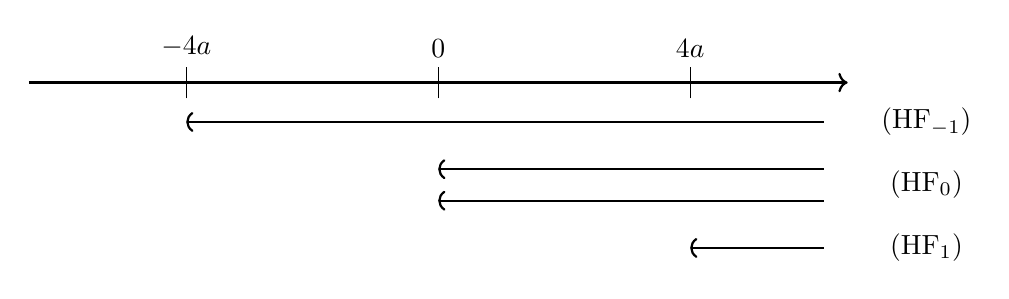
\begin{tikzpicture}
\draw[->,thick] (-5.200,0.000)--(5.200,0.000);
\draw[] (0.000,-0.200)--(0.000,0.200) node[above] {0};
\draw[] (-3.200,-0.200)--(-3.200,0.200) node[above] {$-4a$};
\draw[] (3.200,-0.200)--(3.200,0.200) node[above] {$4a$};
\draw[(-,thick] (-3.200,-0.500)--(4.900,-0.500);
\node[] at (6.200,-0.500) {$(\HF_{-1})$};
\draw[(-,thick] (0.000,-1.100)--(4.900,-1.100);
\draw[(-,thick] (0.000,-1.500)--(4.900,-1.500);
\node[] at (6.200,-1.300) {$(\HF_0)$};
\draw[(-,thick] (3.200,-2.100)--(4.900,-2.100);
\node[] at (6.200,-2.100) {$(\HF_{1})$};
\end{tikzpicture}
\caption{The barcode of the filtered Floer homology of $\phi^2$, for $0<a<2$.}
\end{figure}

For $a = 2$, $\phi^2$ is a degenerate Hamiltonian diffeomorphism.

For $2<a<\pi$, the barcode of $\phi^2$ is given by
\begin{figure}[H]
\centering
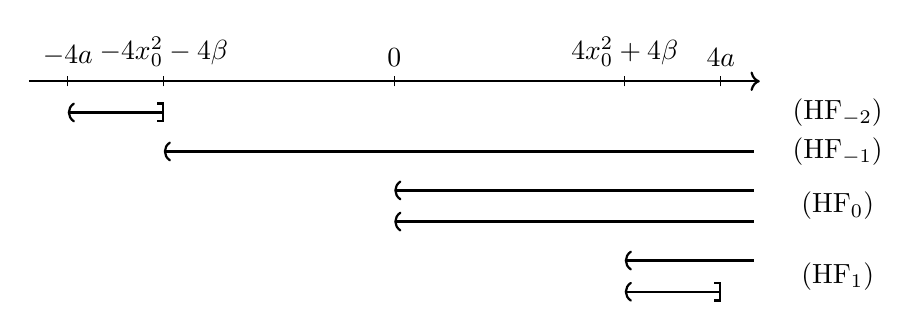
\begin{tikzpicture}[scale=0.33]
\draw[->,thick] (-14.066,0.000)--(14.066,0.000);
\draw[] (0.000,-0.200)--(0.000,0.200) node[above] {0};
\draw[] (-12.566,-0.200)--(-12.566,0.200) node[above] {$-4a$};
\draw[] (12.566,-0.200)--(12.566,0.200) node[above] {$4a$};
\draw[] (-8.870,-0.200)--(-8.870,0.200) node[above] {$-4 x_0^2 - 4 \beta$};
\draw[] (8.870,-0.200)--(8.870,0.200) node[above] {$4 x_0^2 + 4 \beta$};
\draw[{(-]},thick] (-12.566,-1.200)--(-8.870,-1.200) node[right] {};
\node[] at (17.066,-1.200) {$(\HF_{-2})$};
\draw[(-,thick] (-8.870,-2.700)--(13.841,-2.700) node[right] {};
\node[] at (17.066,-2.700) {$(\HF_{-1})$};
\draw[(-,thick] (0.000,-4.200)--(13.841,-4.200) node[right] {};
\draw[(-,thick] (0.000,-5.400)--(13.841,-5.400) node[right] {};
\node[] at (17.066,-4.800) {$(\HF_0)$};
\draw[(-,thick] (8.870,-6.900)--(13.841,-6.900) node[right] {};
\draw[{(-]},thick] (8.870,-8.100)--(12.566,-8.100) node[right] {};
\node[] at (17.066,-7.500) {$(\HF_{1})$};
\end{tikzpicture}
\caption{The barcode of the filtered Floer homology of $\phi^2$, for $2<a<\pi$.}
\end{figure}
\end{theorem}

\begin{corollary}
For $2 < a < \pi$, the Hamiltonian diffeomorphism $\phi$ is not generated by an autonomous Hamiltonian.
\end{corollary}

\begin{proof}
If $\phi$ were generated by an autonomous Hamiltonian, so would $\phi^2$ (as one could flow with the same Hamiltonian in twice the time). Therefore, it suffices to show that $\phi^2$ is not generated by an autonomous Hamiltonian.

Recall that (proposition \ref{maslovmorse}) the Maslov indices of critical points of a Hamiltonian diffeomorphism induced by an autonomous Hamiltonian are all zero or odd. Therefore, the barcode of such a diffeomorphism cannot have any bars in index $-2$, and every bar in index $1$ must only terminate at infinity. Neither of these conditions are satisfied by the barcode of $\phi^2$.

On a slightly more elementary level, the proof boils down to the fact that $\phi^2$ has fixed points ($B_0$ and $B_3$) with Maslov index $\pm 2$.

An alternative proof, more elementary yet, consists of noticing that if $\phi$ were a Hamiltonian diffeomorphism and there was a pair of distinct points $x, y$ satisfying $\phi(x) = y$ and $\phi(y) = x$, then there would be infinitely many pairs of such points: if $\phi$ were the time-one flow of a Hamiltonian diffeomorphism, $x$ and $y$ would be part of a nonconstant time-two periodic orbit, and hence there would be infinitely more such pairs. Now, apply this argument to $(x_0,y_0)$ and $(-x_0,-y_0)$.
\end{proof}



\bibliographystyle{plain}
\bibliography{bibliography}

\end{document}